\chapter{The correspondence between Stokes data and Stokes shells of Gaussian type}

In this chapter, our aim is to establish a correspondence between the category of Stokes shells and the category of Stokes data for differential systems of Gaussian type $\{r,z\} \subseteq \C$, where $r \in \R_{>0}$ and $z\in \C\smallsetminus \R$. Particularly, considering a direction $\theta_0 \in S^1$ that is generic with respect to $C \coloneqq \{r,z\}$, we will prove that there exists an equivalence of categories between $\SD(C,\theta_0)$ and $\SH(C)$. Moreover, we will give a precise description of the involved functors. 

\section{From shells to data}\label{ShellData}
Let $\StSh=((\gr\Lo, \gr\Lo_{\leq \bullet}), \Defo)$ be a Stokes shell of Gaussian type $C \coloneqq \{r,z\}$ with elements $r \in \R_{>0}$ and $z \in \C\smallsetminus\R$.
Since $C \neq -C$ we add $-r,-z$ to $C$ and consider $(\gr\Lo, \gr\Lo_{\leq \bullet})$ of type $\tilde{C}\coloneqq \{r,-r,z,-z\}$. Remark that $\gr_{-r}\Lo = 0$ and $\gr_{-z}\Lo = 0$ because the set of exponential factors of $(\gr\Lo, \gr\Lo_{\leq \bullet})$ is a subset of $C$. 

We start by specifying the notations from the previous chapter to apply to this particular case. For improved readability we use the following notation:
\begin{nota}
    We set
    \begin{itemize}
        \item $\theta_r^{(\nu)} \coloneqq \frac{\pi}{4}+ \nu \frac{\pi}{2} $ for $\nu \in \Z/4\Z$,
        \item $\theta_z^{(\nu)} \coloneqq \frac{\pi+ 2\arg(z)}{4}+ \nu\frac{\pi}{2}$ for $\nu \in \Z/4\Z$ and 
        \item $I_c^{(\nu)} \coloneqq (\theta_{c}^{(\nu)},\theta_{c}^{(\nu+1)}) \subseteq \R/2\pi\Z$ for $\nu \in \Z/4\Z$ and $c \in \{r,z\}$.
    \end{itemize}
\end{nota}

Given that $\St(0,c) = \St(0,-c)$ for all $c \in \C$, we obtain
\begin{itemize}
    \item $S_0(\tilde{C})= \St(0,r) \cup \St(0,z)= \left\{\theta_r^{(\nu)} ~\big\vert~ \nu \in \Z /4\Z\right\} \cup \left\{\theta_z^{(\nu)} ~\big\vert~ \nu \in \Z/4\Z\right\}$. 
    \item $T(\tilde{C}) = \left\{I_r^{(\nu)} ~\big\vert~ \nu \in \Z/4\Z\right\} \cup \left\{I_z^{(\nu)} ~\big\vert~ \nu \in \Z/4\Z\right\}$ and
    \item $\Ac(\tilde{C}) = \bigcup_{\nu \in \Z/4\Z} \left\{(r, I_r^{(\nu)}), (-r, I_r^{(\nu)}), (z, I_z^{(\nu)}), (-z, I_z^{(\nu)}) \right\}$.
\end{itemize}

\begin{figure}[h!]
\centering

\begin{minipage}{0.48\textwidth}
\centering
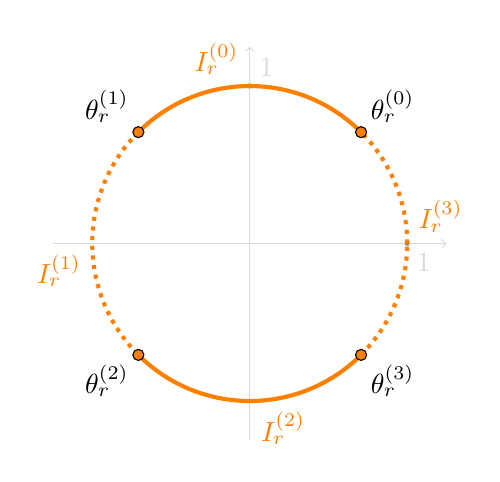
\begin{tikzpicture}
  % Gray coordinate system
  \draw[gray!30,->] (-2.5,0) -- (2.5,0) node[right] {$\re$};
  \draw[gray!30,->] (0,-2.5) -- (0,2.5) node[above] {$\im$};

  \draw[gray!30,fill=gray] (2,0) circle (1pt) node[below right] {1};
  \draw[gray!30,fill=gray] (0,2) circle (1pt) node[above right] {1};

   %Intervals for r
    \draw[orange, line width=1.5pt] (45:2cm) arc (45:135:2cm) node[midway, above left] {$I_r^{(0)}$};
   \draw[orange, dotted, line width=1.5pt] (135:2cm) arc (135:225:2cm) node[midway, below left] {$I_r^{(1)}$};
   \draw[orange, line width=1.5pt] (225:2cm) arc (225:315:2cm) node[midway, below right] {$I_r^{(2)}$};
   \draw[orange, dotted, line width=1.5pt] (315:2cm) arc (315:360:2cm) node[above right] {$I_r^{(3)}$};
   \draw[orange, dotted, line width=1.5pt] (0:2cm) arc (0:45:2cm);
  
  
  % Stokes directions for r
  \draw[fill=orange] (45:2cm) circle (2pt) node[above right] {$\theta_r^{(0)}$};
  \draw[fill=orange] (135:2cm) circle (2pt) node[above left]{$\theta_r^{(1)}$};
  \draw[fill=orange] (225:2cm) circle (2pt) node[below left]{$\theta_r^{(2)}$};
  \draw[fill=orange] (315:2cm) circle (2pt) node[below right]{$\theta_r^{(3)}$};

   
\end{tikzpicture}
\captionsetup{font=small}
\caption{The set $\St(0,r)$ with open intervals $I^{(\nu)}_r$.}
\end{minipage}
\hfill
\begin{minipage}{0.48\textwidth}
\centering
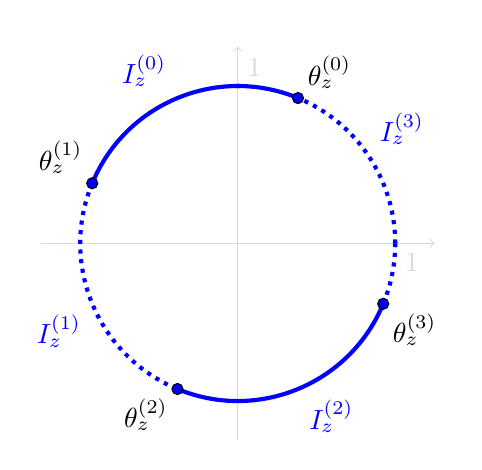
\begin{tikzpicture}
 % coordinate system
  \draw[gray!30,->] (-2.5,0) -- (2.5,0) node[right] {$\re$};
  \draw[gray!30,->] (0,-2.5) -- (0,2.5) node[above] {$\im$};
  \draw[gray!30,fill=gray] (2,0) circle (1pt) node[below right] {1};
  \draw[gray!30,fill=gray] (0,2) circle (1pt) node[above right] {1};

   %Intervals for z
   \draw[blue, line width=1.5pt] (67.5:2cm) arc (67.5:157.5:2.cm) node[midway, above left] {$I_z^{(0)}$};
   \draw[blue, dotted, line width=1.5pt] (157.5:2cm) arc (157.5:247.5:2cm) node[midway, below left] {$I_z^{(1)}$};
   \draw[blue, line width=1.5pt] (247.5:2cm) arc (247.5:337.5:2cm) node[midway, below right] {$I_z^{(2)}$};
   \draw[blue, dotted, line width=1.5pt] (337.5:2cm) arc (337.5:360:2cm);
   \draw[blue, dotted, line width=1.5pt] (0:2cm) arc (0:67.5:2cm) node[midway, above right] {$I_z^{(3)}$};

    % Stokes directions for z
  \draw[fill=blue] (67.5:2cm) circle (2pt) node[above right]{$\theta_z^{(0)}$};
  \draw[fill=blue] (157.5:2cm) circle (2pt) node[above left]{$\theta_z^{(1)}$};
  \draw[fill=blue] (247.5:2cm) circle (2pt) node[below left]{$\theta_z^{(2)}$};
  \draw[fill=blue] (337.5:2cm) circle (2pt) node[below right]{$\theta_z^{(3)}$};
\end{tikzpicture}
\captionsetup{font=small}
\caption{The set $\St(0,z)$ for $\arg(z)=\frac{\pi}{4}$ with open intervals $I^{(\nu)}_z$.}
\end{minipage}
\end{figure}


To describe the deformation datum of a Stokes Shell of Gaussian type, we have to describe $\B_2(\tilde{C})$ and $T_2(\tilde{C})$. Thus we first need to specify $c_+^{I}$ and $c_-^{I}$ for any interval $I \in T(\tilde{C})$. 
\begin{itemize}
    \item For $c \in \{r,z\}$ and for $I \in \{I_c^{(0)},I_c^{(2)}\}$ we get $c_+^{I} = -c, c_-^{I} = c$.
    \item For $c \in \{r,z\}$ and for $I \in \{I_c^{(1)}, I_c^{(3)}\}$ we get $c_+^{I} = c, c_-^{I} = -c$.
\end{itemize}
This yields to
\begin{itemize}
    \item $\B_2(\tilde{C}) =\bigcup_{c \in \{r,z\}} \left\{(-c,c;I_c^{(0)}),(-c,c;I_c^{(2)}),(c,-c;I_c^{(1)}),(c,-c;I_c^{(3)})\right\}$.
\end{itemize}
Describing $T_2(\tilde{C})$ is slightly more complicated, since the intervals $I_z^{(\nu)}$ depend on $\arg(z)$. That is why we first have to make the following observation: 

\begin{lem}\label{lem-nu} Let $C = \{r,z\}$ be a set with $r \in \R_{>0}$ and $z \in \C\smallsetminus \R$. Then there is exactly one Stokes direction $\theta_z^{(\nu_o)} \in \St(0,z)$ with $\theta_z^{(\nu_o)}\mod 2 \pi  \in \left( \frac{\pi}{4}, \frac{3\pi}{4} \right)$.
    More precisely, if $\im(z) > 0$, then $\nu_o = 0$, if $\im(z)<0$, then  $\nu_o = 3$.
\end{lem}
\begin{proof} Let $z\in \C \smallsetminus \R$ be a complex number with $\im(z) \neq 0$.
    If $\im(z)>0$, we have $\arg(z) \in (0,\pi)$. Then 
    \[
    \frac{\arg(z)}{2} \in \left(0, \frac{\pi}{2}\right) \Leftrightarrow \theta_z^{(0)} = \frac{\pi}{4}+\frac{\arg(z)}{2}\in \left(\frac{\pi}{4},\frac{3\pi}{4}\right) = (\theta_r^{(0)}, \theta_r^{(1)}).
    \]
    If $\im(z)<0$, we have $\arg(z) \in (\pi,2\pi)$. Then 
    \begin{align*}
    \frac{\arg(z)}{2} \in \left(\frac{\pi}{2}, \pi\right) & \Leftrightarrow \frac{\pi}{4}+\frac{\arg(z)}{2}\in \left(\frac{3\pi}{4},\frac{5\pi}{4}\right) \\ &  \Leftrightarrow \theta_z^{(3)}=\frac{\pi}{4}+\frac{\arg(z)}{2} + \frac{3\pi}{2} \in \left(\frac{9\pi}{4},\frac{11\pi}{4}\right) \\ & \Rightarrow  \theta_z^{(3)} \mod 2\pi \in \left(\frac{\pi}{4},\frac{3\pi}{4}\right)= (\theta_r^{(0)}, \theta_r^{(1)}).
    \end{align*}
    In both cases there is only one Stokes direction $\theta_z^{(\nu_o)}$ with $\theta_z^{(\nu_o)} \mod 2\pi \in (\theta_r^{(0)}, \theta_r^{(1)})$, since the elements in $\St(0,z)$ differ by a multiple of $\frac{\pi}{2}$ and $(\theta_r^{(0)}, \theta_r^{(1)})$ is an open interval of length $\frac{\pi}{2}$.
\end{proof}

Using (\ref{lem-nu}) we can describe $T_2(\tilde{C})$.
\begin{enumerate}
    \item If $\im(z)>0$, then $I_r^{(\nu)}$ has non-empty intersection with $I_z^{(\nu)}$ and with $I_z^{(\nu+3)}$, because $\theta_z^{(\nu)} \in I_r^{(\nu)}$. Moreover $I_r^{(\nu)} \cap I_z^{(\nu+1)}=\varnothing$ and $I_r^{(\nu)}\cap I_z^{(\nu+2)} = \varnothing$. This results in  \[ T_2(\tilde{C}) = \bigcup_{\nu \in \Z/4\Z} \left\{(I_r^{(\nu)},I_z^{(\nu)}),(I_z^{(\nu)}, I_r^{(\nu)}),(I_r^{(\nu)},I_z^{(\nu+3)}), (I_z^{(\nu+3)}, I_r^{(\nu)})\right\}.\]
    \item Analogously if $\im(z) < 0$ we get $I_r^{(\nu)} \cap I_z^{(\nu+2)} \neq \varnothing, I_r^{(\nu)} \cap I_z^{(\nu+3)} \neq \varnothing$ and $I_r^{(\nu)} \cap I_z^{(\nu)} = \varnothing, I_r^{(\nu)} \cap I_z^{(\nu+1)} = \varnothing$, because $\theta_z^{(\nu+3)} \in I_r^{(\nu)}$. This results in
    \[T_2(\tilde{C}) = \bigcup_{\nu \in \Z/4\Z} \left\{(I_r^{(\nu)},I_z^{(\nu+2)}),(I_z^{(\nu+2)}, I_r^{(\nu)}),(I_r^{(\nu)},I_z^{(\nu+3)}), (I_z^{(\nu+3)}, I_r^{(\nu)})\right\}.\]
\end{enumerate}


In order to describe the deformation datum $\Defo$, it is essential to outline the Stokes tuple of $\k$-vector spaces $\mathfrak{D}((\gr\Lo, \gr\Lo_{\leq \bullet}))$ that is induced by $(\gr\Lo,\gr\Lo_{\leq \bullet})$. 

As we saw in the previous chapter (lemma \ref{gradedtotupel}), $\mathfrak{D}((\gr\Lo, \gr\Lo_{\leq \bullet}))=(\K, \bm{\Phi},\bm{\Psi})$ with $\K \coloneqq (K_{c,I_c^{(\nu)}})_{(c,I_c^{(\nu)}) \in \Ac(\tilde{C})}$, $\bm\Phi \coloneqq (\Phi_c^{(\nu+1,\nu)})_{(c,I_c^{(\nu)}) \in \Ac(\tilde{C})}$ and $\bm\Psi \coloneqq (\Psi_{c,I_c^{(\nu)}})_{(c,I_c^{(\nu)}) \in \Ac(\tilde{C})}$ where 
\begin{itemize}
    \item $K_{c,I_c^{(\nu)}} \coloneqq \gr_c\Lo(\overline{I_c^{(\nu)}})$,
    \item $\Phi_c^{(\nu+1,\nu)}:K_{c, I^{(\nu)}_c} \to K_{c,I^{(\nu+1)}_c}$ is given by $\gr_c\Lo(\overline{I^{(\nu)}_c}) \cong \gr_c\Lo_{\theta_c^{(\nu+1)}} \cong \gr_c\Lo(\overline{I_c^{(\nu+1)}})$
    \item and $\Psi_{c,I^{(\nu)}_c} = \id_{K_{c,I_c^{(\nu)}}}:K_{c,I_c^{(\nu)}} \to K_{c,I_c^{(\nu)}}$.
\end{itemize}

Given that $(\gr\Lo, \gr\Lo_{\leq \bullet})$ is of type $C=\{r,z\}$ for $c \in \{-r,-z\}$ and $\nu \in \Z/4\Z$, we obtain $K_{c,I_c^{(\nu)}}= \gr_c\Lo(\overline{I^{(\nu)}_c}) =0$.



By definition (\ref{Defo}), $\Defo$ consists of 
\begin{itemize}
    \item a morphism $\Rc_{I_1}^{I_2}:K_{c_+^{I_1},I_1} \to K_{c_-^{I_2},I_2}$ for each pair $(I_1, I_2) \in T_2(\tilde{C})$ and
    \item a morphism $\Rc_{c_2, I_+}^{c_1, I_-}: K_{c_1, I} \to K_{c_2, I}$ for each tuple $(c_1,c_2;I) \in \B_2(\tilde{C})$.
\end{itemize}

First we notice, that for any given tuple $(c_1,c_2;I) \in \B_2(\tilde{C})$ either $c_1 \in \{-r,-z\}$ or $c_2 \in \{-r,-z\}$ and therefore $K_{c_1,I}=0$ or $K_{c_2,I}=0$, so $\Rc_{c_2, I_+}^{c_1, I_-}$ is the zero morphism.

In order to specify $\Rc_{I_1}^{I_2}$ for a given pair $(I_1,I_2) \in T_2(\tilde{C})$ notice that if $I_1 \in \{I_c^{(0)}, I_c^{(2)}\}$ or $I_2 \in \{I_c^{(1)}, I_c^{(3)}\}$ for some $c \in C$ the morphism $\Rc_{I_1}^{I_2}$ is the zero morphism as $c_{-}^{I_c^{(1)}} = c_-^{I_c^{(3)}}=-c$, and $c_+^{I_c^{(0)}}=c_+^{I_c^{(2)}}=-c$. 

Consequently, the deformation datum $\Defo$ is given by four linear morphisms:
    \begin{multicols}{2} % Start the two-column layout
    \begin{enumerate}
        \item $\Rc_0 \coloneqq \Rc_{I_z^{(3)}}^{I_r^{(0)}}:K_{z,I_z^{(3)}} \to K_{r,I_r^{(0)}}$,
        \item $\Rc_1 \coloneqq \Rc_{I_r^{(1)}}^{I_z^{(0)}}: K_{r, I_r^{(1)}} \to K_{z,I_z^{(0)}}$,
        \item $\Rc_2 \coloneqq \Rc_{I_z^{(1)}}^{I_r^{(2)}}: K_{z,I_z^{(1)}} \to K_{r,I_r^{(2)}}$,
        \item $\Rc_3 \coloneqq \Rc_{I_r^{(3)}}^{I_z^{(2)}}: K_{r, I_r^{(3)}} \to K_{z,I_z^{(2)}}$. 
    \end{enumerate}
    \end{multicols}

    
\begin{comment}
\begin{rem}
    Ist ein Morphismus $\Rc_{I_1}^{I_2}$ mit $I_1 = I_r^{(\nu_r)}$; $I_2 =I_z^{(\nu_z)}$ aus $\Defo$ nicht trivial, dann gilt $r \geq_\theta z$ für alle $\theta \in I_1 \cap I_2$, denn für $\theta \in I_1$ gilt $r \geq_\theta 0 $ und für $\theta \in I_2$ gilt $0 \geq_\theta z$. Analog natürlich für $I_1 = I_z^\bullet$, $I_2 = I_r^\bullet$.
\end{rem}
\end{comment}

Having seen that in our context $\Defo$ can be described by four morphisms, we can take the next step and show that each Stokes shell of Gaussian type $C$ can be viewed as an object in $\SD(C,\theta_0)$. 

\begin{lem}\label{shelltodata}
    Consider $C=\{r,z\}$ with $r \in \R_{>0}$, $z \in \C \smallsetminus \R$ and let $\theta_0 \in S^1$ be a generic direction with respect to $C$. A Stokes shell of Gaussian type $C$ induces an object in $\SD(C,\theta_0)$.
\end{lem}
\begin{proof} 
    Let $\StSh =((\gr\Lo, \gr\Lo_{\leq \bullet}),\Defo)$ be a Stokes shell of Gaussian type $C$, and $\mathfrak{D}((\gr\Lo, \gr\Lo_{\leq \bullet})) = (\K, \bm{\Phi},\bm{\Psi})$. Then $\Defo$ is given by 
    \begin{multicols}{2} % Start the two-column layout
        \begin{enumerate}
        \item $\Rc_0 \coloneqq \Rc_{I_z^{(3)}}^{I_r^{(0)}}:K_{z,I_z^{(3)}} \to K_{r,I_r^{(0)}}$,
        \item $\Rc_1 \coloneqq \Rc_{I_r^{(1)}}^{I_z^{(0)}}: K_{r, I_r^{(1)}} \to K_{z,I_z^{(0)}}$,
        \item $\Rc_2 \coloneqq \Rc_{I_z^{(1)}}^{I_r^{(2)}}: K_{z,I_z^{(1)}} \to K_{r,I_r^{(2)}}$,
        \item $\Rc_3 \coloneqq \Rc_{I_r^{(3)}}^{I_z^{(2)}}: K_{r, I_r^{(3)}} \to K_{z,I_z^{(2)}}$. 
    \end{enumerate}
    \end{multicols} % End the two-column layout
    Set $G_r^{(\nu)}\coloneqq K_{r,I_r^{(\nu)}}=\gr_r\Lo(\overline{I_r^{(\nu)}})$ and $G_z^{(\nu)}\coloneqq K_{z,I_z^{(\nu+3)}}=\gr_z\Lo(\overline{I_z^{(\nu+3)}})$ for each $\nu \in \Z/4\Z$.
    
    Since $\theta_0$ is generic with respect to $C$, we either have $r \leq_{\theta_0} z$ or $z \leq_{\theta_0} r$. So we distinguish between the two cases:
    \begin{enumerate}
        \item Consider the case $r \leq_{\theta_0} z$, so the unique numbering of $C$ given by $\theta_0$ is $c_1 = r$, $c_2 = z$. Set 
        \begin{align*}
            S^{(1,0)} & \coloneqq 
        \begin{pmatrix}
            \Phi^{(1,0)}_r & 0\\
              \Rc_1 \circ \Phi_r^{(1,0)}& \Phi_z^{(0,3)}
        \end{pmatrix},~
        S^{(2,1)} \coloneqq 
        \begin{pmatrix}
            \Phi^{(2,1)}_r &  \Rc_2 \circ \Phi^{(1,0)}_z\\
            0 & \Phi_z^{(1,0)}
        \end{pmatrix}, \\
         S^{(3,2)} & \coloneqq 
        \begin{pmatrix}
            \Phi^{(3,2)}_r & 0\\
             \Rc_3 \circ \Phi_r^{(3,2)} & \Phi_z^{(2,1)}
        \end{pmatrix},~
        S^{(0,3)} \coloneqq 
        \begin{pmatrix}
            \Phi^{(0,3)}_r & \Rc_0 \circ \Phi^{(3,2)}_z\\
           0 & \Phi_z^{(3,2)}
        \end{pmatrix}.
        \end{align*}
        Then $((G_c^{(\nu)})_{c \in C}, S^{(\nu+1,\nu)})_{\nu \in \Z/4\Z}$ is an object in $\SD(C,\theta_0)$, since $\bm{\Phi}$ is a tuple of isomorphisms, $S^{(1,0)},S^{(3,2)}$ are block-lower and $S^{(2,1)},S^{(0,3)}$ are block-upper triangular. We can illustrate $((G_c^{(\nu)})_{c \in C}, S^{(\nu+1,\nu)})_{\nu \in \Z/4\Z}$ in the following diagram:
        \[
         \begin{tikzcd}[row sep=1cm, column sep=0cm]
         & K_{r,I_r^{(0)}} \oplus K_{z,I_z^{(3)}} \arrow[dl, "S^{(1,0)}"'] & \\
        K_{r,I_r^{(1)}} \oplus K_{z,I_z^{(0)}} \arrow[dr, "S^{(2,1)}"'] & & K_{r,I_r^{(3)}} \oplus K_{z,I_z^{(2)}} \arrow[ul, "S^{(0,3)}" above right] \\
        & K_{r,I_r^{(2)}} \oplus K_{z,I_z^{(1)}}\arrow[ur, "S^{(3,2)}" below right] &
        \end{tikzcd}
        \]
    \item Consider the case $z \leq_{\theta_0} r$, then the unique numbering of $C$ given by $\theta_0$ is $c_1 = z$, $c_2 = r$. Setting 
        \begin{align*}
            S^{(1,0)} & \coloneqq 
        \begin{pmatrix}
            \Phi^{(0,3)}_z & 0\\
            \Phi_r^{(1,0)} \circ \Rc_0 & \Phi_r^{(1,0)}
        \end{pmatrix},~
        S^{(2,1)} \coloneqq 
        \begin{pmatrix}
            \Phi^{(1,0)}_z & \Phi^{(1,0)}_z \circ \Rc_1 \\
            0 & \Phi_r^{(2,1)}
        \end{pmatrix}, \\
         S^{(3,2)} & \coloneqq 
        \begin{pmatrix}
            \Phi^{(2,1)}_z & 0 \\
            \Phi_r^{(3,2)} \circ \Rc_2 & \Phi_r^{(3,2)}
        \end{pmatrix},~
        S^{(0,3)} \coloneqq 
        \begin{pmatrix}
            \Phi^{(3,2)}_z & \Phi_z^{(3,2)}\circ \Rc_3 \\
            0 & \Phi_r^{(0,3)}
        \end{pmatrix},
        \end{align*}
        defines an object $((G_c^{(\nu)})_{c \in C}, S^{(\nu+1,\nu)})_{\nu \in \Z/4\Z}$ in $\SD(C,\theta_0)$, since $\bm{\Phi}$ is a tuple of isomorphisms, $S^{(1,0)},S^{(3,2)}$ are block-lower and $S^{(2,1)},S^{(0,3)}$ are block-upper triangular. We can illustrate $((G_c^{(\nu)})_{c \in C}, S^{(\nu+1,\nu)})_{\nu \in \Z/4\Z}$ in the following diagram:
        \[
         \begin{tikzcd}[row sep=1cm, column sep=0cm]
         & K_{z,I_z^{(3)}} \oplus K_{r,I_r^{(0)}} \arrow[dl, "S^{(1,0)}"'] & \\
        K_{z,I_z^{(0)}} \oplus K_{r,I_r^{(1)}} \arrow[dr, "S^{(2,1)}"'] & & K_{z,I_z^{(2)}} \oplus K_{r,I_r^{(3)}} \arrow[ul, "S^{(0,3)}" above right] \\
        & K_{z,I_z^{(1)}} \oplus K_{r,I_r^{(2)}}\arrow[ur, "S^{(3,2)}" below right] &
        \end{tikzcd}
        \]
\end{enumerate}
Thus in both cases we get an object in $\SD(C,\theta_0)$.
\end{proof}

Next we will show that this extends to a functor $\SH(C) \to \SD(C,\theta_0)$.


\begin{prop}\label{F-functor}
    Consider $C=\{r,z\}$ with $r \in \R_{>0}$ and $z \in \C\smallsetminus \R$ and let $\theta_0 \in S^1$ be a generic direction with respect to $C$. Define 
    \[
    \begin{matrix}
        F_{\theta_0}: & \SH(C) &\longrightarrow & \SD(C,\theta_0), \\
        & \StSh &\longmapsto & F_{\theta_0}(\StSh)
    \end{matrix}
    \]
    where $F_{\theta_0}(\StSh) \coloneqq ((G_c^{(\nu)})_{c \in C}, S^{(\nu+1,\nu)})_{\nu \in \Z/4\Z}$ is the Stokes data induced by $\StSh$ as defined in lemma (\ref{shelltodata}). Then $F_{\theta_0}$ is a functor between $\SH(C)$ and $\SD(C,\theta_0)$.
\end{prop}

\begin{proof}
    First we have to define $F_{\theta_0}$ on $\Hom_{\SH(C)}(\StSh, \tilde{\StSh})$. Let $\lambda \in \Hom_{\SH(C)}(\StSh, \tilde{\StSh})$, $F_{\theta_0}(\StSh) \coloneqq ((G_c^{(\nu)})_{c \in C}, S^{(\nu+1,\nu)})_{\nu \in \Z/4\Z}$ and $F_{\theta_0}(\tilde{\StSh}) \coloneqq ((\tilde{G}_c^{(\nu)})_{c \in C}, \tilde{S}^{(\nu+1,\nu)})_{\nu \in \Z/4\Z}$. 
    
    Since
    \[
    \lambda: \gr\Lo = \gr_r\Lo \oplus \gr_z\Lo \to \gr_r\tilde{\Lo} \oplus \gr_z\tilde{\Lo}=\gr\tilde{\Lo}
    \] is a graded morphism, in particular one has $\lambda(\overline{I_c^{(\nu)}})(\gr_c\Lo(\overline{I_c^{(\nu)}})) \subseteq \gr_c\tilde{\Lo}(\overline{I_c^{(\nu)}})$. Thus for each $(c,I_c^{(\nu)}) \in \Ac(C)$ we get a morphism of vector spaces 
    \[
    \lambda_c^{(\nu)}\coloneqq \lambda(\overline{I_c^{(\nu)}})\vert_{\gr_c\Lo(\overline{I_c^{(\nu)}})}:\gr_c\Lo(\overline{I_c^{(\nu)}}) \to \gr_c\tilde{\Lo}(\overline{I_c^{(\nu)}}).
    \]
    Define
    \[
    \begin{matrix}
        \lambda^{(\nu)}: & \gr_r\Lo(\overline{I_r^{(\nu)}}) \oplus \gr_z\Lo(\overline{I_z^{(\nu+3)}}) & \longrightarrow & \gr_r\tilde{\Lo}(\overline{I_r^{(\nu)}}) \oplus \gr_z\tilde{\Lo}(\overline{I_z^{(\nu+3)}}) \\
        &(x, y) &\longmapsto  &(\lambda_r^{(\nu)}(x), \lambda_z^{(\nu+3)}(y))
    \end{matrix}.
    \]
    
    Then $(\lambda^{(\nu)})_{\nu \in \Z/4\Z} \in \Hom_{\SD(C,\theta_0)}(F_{\theta_0}(\StSh),F_{\theta_0}(\tilde{\StSh}))$, because if writing \[\lambda^{(\nu)} = (\lambda_{ij}^{(\nu)}: G_{c_j}^{(\nu)} \to \tilde{G}_{c_i}^{(\nu)})_{c_i,c_j \in \{r,z\}},\] then $\lambda_{ij}^{(\nu)} = 0$ if $i\neq j$ and if $r \leq_{\theta_0} z$ and $\nu \in \{1,3\}$: 
        \begin{align*}
\tilde{S}^{(\nu+1,\nu)} \lambda^{(\nu)} & = 
        \begin{pmatrix}
            \tilde{\Phi}^{(\nu+1,\nu)}_r & \tilde{\Rc}_{\nu+1}\tilde{\Phi}_z^{(\nu,\nu+3)}\\
            0 & \tilde{\Phi}_z^{(\nu,\nu+3)}
        \end{pmatrix} 
        \begin{pmatrix}
            \lambda_r^{(\nu)} & 0\\
            0 & \lambda_z^{(\nu+3)}
        \end{pmatrix}
        \\ & =
        \begin{pmatrix}
            \tilde{\Phi}^{(\nu+1,\nu)}_r \lambda_r^{(\nu)} & \tilde{\Rc}_{\nu+1 }\tilde{\Phi}_z^{(\nu,\nu+3)} \lambda_z^{(\nu+3)}\\
            0 & \tilde{\Phi}_z^{(\nu,\nu+3)}\lambda_z^{(\nu+3)}
        \end{pmatrix} 
        \\ & \overset{(1)}{=} \begin{pmatrix}
            \lambda_r^{(\nu+1)}\Phi^{(\nu+1,\nu)}_r & \tilde{\Rc}_{\nu+1}\lambda_z^{(\nu)}\Phi_z^{(\nu,\nu+3)}\\
            0 & \lambda_z^{(\nu)}\Phi_z^{(\nu,\nu+3)}
        \end{pmatrix}
        \\ & \overset{(2)}{=}
        \begin{pmatrix}
            \lambda_r^{(\nu+1)} \Phi^{(\nu+1,\nu)}_r &  \lambda_z^{(\nu)}\Rc_{\nu+1}\Phi_z^{(\nu,\nu+3)}\\
            0 & \lambda_z^{(\nu)}\Phi_z^{(\nu,\nu+3)}
        \end{pmatrix} 
        \\ & = 
        \begin{pmatrix}
            \lambda_r^{(\nu+1)} & 0\\
            0 & \lambda_z^{(\nu)}
        \end{pmatrix} 
        \begin{pmatrix}
            \Phi^{(\nu+1,\nu)}_r & \Rc_{\nu+1}\Phi_z^{(\nu,\nu+3)}\\
            0 & \Phi_z^{(\nu,\nu+3)}
        \end{pmatrix} 
        = \lambda^{(\nu+1)}S^{(\nu+1,\nu)}
\end{align*}
where (1) holds, as $\lambda$ is an morphism of sheaves and $\Phi, \tilde{\Phi}$ are given by the restriction morphisms of the sheaves $\gr\Lo$, $\gr\tilde{\Lo}$ and (2) holds, as $\lambda$ is compatible with the deformation datum. The same arguments show that $\tilde{S}^{(\nu+1,\nu)} \lambda^{(\nu)}=\lambda^{(\nu+1)}S^{(\nu+1,\nu)}$ for $\nu \in \{0,2\}$ and also in the in the setting $z \leq_{\theta_0} r$.

We set $F_{\theta_0}(\lambda) \coloneqq ((\lambda^{(\nu)})_{\nu \in \Z/4\Z})$. Then by definition of $F_{\theta_0}$ on morphisms, $F_{\theta_0}(\id_{\StSh})=\id_{F_{\theta_0}(\StSh)}$ and for morphisms $\lambda \in \Hom_{\SH(C)}(\StSh_1, \StSh_2)$ and $\mu \in \Hom_{\SH(C)}(\StSh_2, \StSh_3)$ we have
\begin{align*}
F_{\theta_0}(\mu \circ \lambda) & = \left(\begin{pmatrix}
            \mu_{r}^{(\nu)} \lambda_r^{(\nu)} & 0\\
            0 & \mu_z^{(\nu+3)} \lambda_z^{(\nu+3)}
        \end{pmatrix}^{(\nu)}\right)_{\nu \in \Z/4\Z} \\ & = 
        \left(\begin{pmatrix}
            \mu_r^{(\nu)} & 0\\
            0 & \mu_z^{(\nu+3)}
        \end{pmatrix}
        \begin{pmatrix}
            \lambda_r^{(\nu)} & 0 \\ 
            0 &  \lambda_{z}^{(\nu+3)}
        \end{pmatrix}
        ^{(\nu)}\right)_{\nu \in \Z/4\Z} \\ & = F_{\theta_0}(\mu) \circ F_{\theta_0}(\lambda).
\end{align*}
Thus, $F_{\theta_0}$ is indeed a functor between $\SH(C)$ and $\SD(C,\theta_0)$.
\end{proof}

Having established a functor from Stokes shells to Stokes data, we will continue with determining a functor from Stokes data to Stokes shells in the next section.

\section{From data to shells}
 To receive a Stokes shell of Gaussian type $C$ for each object in $\SD(C,\theta_0)$, we first have to get a graded Stokes filtered local system as defined in (\ref{gradedLoSysDef}).

\begin{lem}\label{data-to-graded}
    Let $\theta_0 \in S^1$ be generic direction with respect to $C=\{r,z\}$ with $r \in \R_{>0}$ and $z \in \C \smallsetminus \R$. Each object $\sigma =((G_c^{(\nu)})_{c \in C}, S^{(\nu+1,\nu)})_{\nu \in \Z/4\Z}$ in $\SD(C,\theta_0)$ induces a graded Stokes filtered local system that we note with $\mathfrak{L}(\sigma)$.
\end{lem}

\begin{proof} Let $\sigma =((G_c^{(\nu)})_{c \in C}, S^{(\nu+1,\nu)})_{\nu \in \Z/4\Z}$ be an arbitrary object in $\SD(C,\theta_0)$. We will write $S^{(\nu+1,\nu)} = (S_{c_2c_1}^{(\nu+1,\nu)} : G_{c_1}^{(\nu)} \to G_{c_2}^{(\nu+1)})_{c_1,c_2 \in C}$. By definition of $\SD(C,\theta_0)$, $S_{cc}^{(\nu+1,\nu)}$ is an isomorphism for each $c \in C, \nu \in \Z/4\Z$. We set $\theta_\nu \coloneqq \theta_0 + \nu\frac{\pi}{2}$ and $I^{(\nu)}\coloneqq (\theta_\nu, \theta_{\nu+1})$. 

Since $\theta_0$ is a generic direction with respect to $C$, for each $\nu \in \Z/4\Z$ the closed interval $\overline{I^{(\nu)}}$ is $C$-good, precisely there are no Stokes directions on the boundary of the interval. Thus there exists an $\epsilon>0$ with $\epsilon < \frac{\pi}{4}$, such that for any $\nu\in \Z/4\Z$ the open interval $I^{(\nu)}_\epsilon \coloneqq (\theta_\nu - \epsilon, \theta_{\nu+1} + \epsilon)$ contains exactly one Stokes direction of $\St(r,z)$. Besides, $(I^{(\nu)}_\epsilon)_{\nu \in \Z/4\Z}$ is an open cover of $S^1$. 


For each $c \in C$ and $\nu \in \Z/4\Z$ we define
\[
\gr_c\Lo_{I^{(\nu)}_\epsilon} \coloneqq \underline{G_c^{(\nu)}}_{I^{(\nu)}_\varepsilon}
\]
to be the constant sheaf with fiber $G_c^{(\nu)}$ on $I^{(\nu)}_\varepsilon$.
On the intersection $I_\epsilon^{(\nu)} \cap I_\epsilon^{(\nu+1)}$ we get an isomorphism of sheaves \[\phi_c^{(\nu+1,\nu)}: \gr_c\Lo_{I_\epsilon^{(\nu)}}\vert_{I_\epsilon^{(\nu)} \cap I_\epsilon^{(\nu+1)}} \to \gr_c\Lo_{I_\epsilon^{(\nu+1)}}\vert_{I_\epsilon^{(\nu)} \cap I_\epsilon^{(\nu+1)}}\]
that is given by 
\[
\phi_c^{(\nu+1,\nu)}(U): \gr_c\Lo_{I_\epsilon^{(\nu)}}(U) \cong G_c^{(\nu)}  \overset{S_{cc}^{(\nu+1,\nu)}}{\to} G_c^{(\nu+1)} \cong \gr_c\Lo_{I_\epsilon^{(\nu+1)}}(U)
\]
for each open, connected subset $U \subseteq I_\epsilon^{(\nu)} \cap I_\epsilon^{(\nu+1)} = (\theta_{\nu+1}-\epsilon, \theta_{\nu+1}+\epsilon)$.

Via the isomorphisms $(\phi_c^{(\nu+1,\nu)})_{\nu \in \Z/4\Z}$ the sheaves $(\gr_c\Lo_{I_\epsilon^{(\nu)}})_{\nu \in \Z/4\Z}$ glue together to a sheaf $\gr_c\Lo$ on $S^1$ that can be described by 
\[
\gr_c\Lo(U) = \left\{(s_\nu) \in \prod_{\nu \in \Z/4\Z} \gr_c\Lo_{I_\epsilon^{(\nu)}}(U \cap I_\epsilon^{(\nu)}) ~\Big\vert~ \phi_c^{(\nu+1,\nu)}(W)(s_{\nu\vert_{W}}) = s_{\nu+1\vert_{W}}  \right\}
\]
with $W \coloneqq U \cap I^{(\nu)}_\epsilon \cap I_\epsilon^{(\nu+1)}$ (see \ref{gluedsheaf}).
 Remark that we do not need to check the cocycle relation, because there are no triple intersections in the cover $(I_\epsilon^{(\nu)})_{\nu \in \Z/4\Z}$ of $S^1$ as $\epsilon<\frac{\pi}{4}$. The sheaf $\gr_c\Lo$ is locally constant, i.e.\ a local system on $S^1$. 
We get a graded Stokes filtered local system $(\gr\Lo,\gr\Lo_{\leq \bullet})$ of Gaussian type $C$ by setting 

\[\gr\Lo \coloneqq \gr_r\Lo \oplus \gr_c\Lo\]
and for any $c \in \C$ 
\[\gr\Lo_{\leq c} \coloneqq \beta_{r\leq c}(\gr_r\Lo) \oplus \beta_{z \leq c}(\gr_z\Lo).\]
 We set $\mathfrak{L}(\sigma) \coloneqq (\gr\Lo, \gr\Lo_{\leq \bullet})$ to be the induced graded Stokes filtered local system.
\end{proof}

Next, we have to define a deformation datum $\Defo$ for $\mathfrak{L}(\sigma)$. We will use the same notation as in section (\ref{ShellData}), that is 
\begin{itemize}
    \item $\theta_r^{(\nu)} = \frac{\pi}{4}+\nu\frac{\pi}{2}$ for $\nu \in \Z/4\Z$,
    \item $\theta_z^{(\nu)} = \frac{\pi+2\arg(z)}{4}+\nu\frac{\pi}{2} \mod 2\pi$ for $\nu \in \Z/4\Z$ and 
    \item $I_c^{(\nu)} = (\theta_c^{(\nu)}, \theta_c^{(\nu+1)})$ for $\nu \in \Z/4\Z$ and $c \in \{r,z\}$.
\end{itemize} For $\mathfrak{L}(\sigma)$ we get the induced Stokes tuple of $\k$-vector spaces of Gaussian type $\mathfrak{D}(\mathfrak{L}(\sigma)) =(\K,\bm\Phi,\bm\Psi)$ that is given by
\begin{itemize}
    \item $K_{c,I_c^{(\nu)}} \coloneqq \gr_c\Lo(\overline{I_c^{(\nu)}})$ for each pair $(c,I_c^{(\nu)})\in \Ac(\tilde{C})$,
    \item $\Phi_c^{(\nu+1,\nu)}:K_{c, I^{(\nu)}_c} \to K_{c,I^{(\nu+1)}_c}$ from $\gr_c\Lo(\overline{I^{(\nu)}_c}) \cong \gr_c\Lo_{\theta_c^{(\nu+1)}} \cong \gr_c\Lo(\overline{I_c^{(\nu+1)}})$ for each pair $(c,I_c^{(\nu)}) \in \Ac(\tilde{C})$ and
    \item $\Psi_{c,I_c^{(\nu)}} = \id_{K_{c,I_c^{(\nu)}}}:K_{c,I_c^{(\nu)}} \to K_{c,I_c^{(\nu)}}$.
\end{itemize}

To define a deformation datum $\Defo$ for $\mathfrak{L}(\sigma)$ we give a precise description of the vector spaces ($\gr_c\Lo(\overline{I_c^{(\nu)}}))_{c \in C, \nu \in \Z/4\Z}$ first. 
\begin{comment}
Writing $S^{(\nu+1,\nu)} = (S_{c_1c_2}^{(\nu+1,\nu)}:G_{c_2}^{(\nu)} \to G_{c_1}^{(\nu+1)})_{c_1,c_2 \in C}$, then for $r \in C$ we get 
\[
\gr_r\Lo(\overline{I_r^{(0)}}) = \left\{(s_{\nu}) \in \prod_{\nu =1}^3 \gr_r\Lo_{\overline{I^{(\nu)}}}(\overline{I_r^{(0)}}\cap I^{(\nu)}_{\epsilon}) \mid S_{rr}^{(\nu+1,\nu)} ([s_\nu]) = [s_{\nu+1}] \text{ for all } \nu \in \Z/4\Z\right\}
\]
where 

\begin{align*} [s_{\nu}] & \coloneqq s_\nu\vert_{\overline{I_r^{(0)}} \cap \overline{I^{(\nu)}} \cap \overline{I^{(\nu+1)}}} \in \begin{cases} 0 &\text{ if } \theta_{\nu+1} \not\in \overline{I_r^{(0)}} \\
(\gr_c\Lo_{I^{(\nu)}})_{\theta_{\nu+1}} = G_c^{(\nu)} &\text{ if } \theta_{\nu+1} \in \overline{I_r^{(0)}}
\end{cases} \text{ and } \\
[s_{\nu+1}] & \coloneqq s_{\nu+1}\vert_{\overline{I_r^{(0)}} \cap \overline{I^{(\nu)}} \cap \overline{I^{(\nu+1)}}} \in \begin{cases} 0 &\text{ if } \theta_{\nu+1} \not\in \overline{I_r^{(0)}} \\
(\gr_c\Lo_{I^{(\nu+1)}})_{\theta_{\nu+1}} = G_c^{(\nu+1)} &\text{ if } \theta_{\nu+1} \in \overline{I_r^{(0)}}
\end{cases}.
\end{align*}
\end{comment}

Let $(I_\epsilon^{(\nu)})_{\nu \in \Z/4\Z}$ be the open covering of $S^1$ as in the proof of lemma (\ref{data-to-graded}).
The interval $\overline{I_r^{(0)}} = [\frac{\pi}{4},\frac{3\pi}{4}]$ has length $\frac{\pi}{2}$. Since all intervals of the open covering $(I_\epsilon^{(\nu)})_{\nu \in \Z/4\Z}$ have length $\frac{\pi}{2}+2\epsilon$ with $0<\epsilon<\frac{\pi}{4}$, $\overline{I_r^{(0)}} \cap I_\epsilon^{(\nu)}$ is a connected set or it is empty. 
Let $\nu_o \in \Z/4\Z$ be such that $\theta_{\nu_o} \in [0, \frac{\pi}{2}) \mod 2\pi$, then 
\begin{itemize}
    \item $\overline{I_r^{(0)}} \cap I_\epsilon^{(\nu_o)} \neq \varnothing$, so $\gr_r\Lo_{I_\epsilon^{(\nu_o)}}(\overline{I_r^{(0)}} \cap I_\epsilon^{(\nu_o)}) = G_r^{(\nu_o)}$ and 
    \item $\overline{I_r^{(0)}} \cap I_\epsilon^{(\nu_o+2)} = \varnothing$, so $\gr_r\Lo_{I_\epsilon^{(\nu_o)}}(\overline{I_r^{(0)}} \cap I_\epsilon^{(\nu_o+2)}) = 0$.
\end{itemize}
The intersections of the intervals $I^{(\nu_o+1)}_\epsilon, I^{(\nu_o+3)}_{\epsilon}$ with $\overline{I_r^{(0)}}$ depend on $\epsilon$ and $\theta_{\nu_o}$. Nevertheless, we can give a precise description of $\gr_r\Lo(\overline{I_r^{(0)}})$ distinguishing the different cases that may occur:
\begin{enumerate}
    \item If $I_\epsilon^{(\nu_o+1)} \cap \overline{I_r^{(0)}} \neq \varnothing$ and $I_\epsilon^{(\nu_o+3)} \cap \overline{I_r^{(0)}} = \varnothing$, then we get
    \[
    \gr_r\Lo(\overline{I_r^{(0)}}) = \left\{(s_{\nu_o}, s_{\nu_o+1}) \in G_r^{(\nu_o)} \times G_r^{(\nu_o+1)} \mid S_{rr}^{(\nu_o+1,\nu_o)}(s_{\nu_o}) = s_{\nu_o+1} \right\}.
    \] 
    \item If $I_\epsilon^{(\nu_o+1)} \cap \overline{I_r^{(0)}} = \varnothing$ and $I_\epsilon^{(\nu_o+3)} \cap \overline{I_r^{(0)}} \neq \varnothing$, then we get
    \[
    \gr_r\Lo(\overline{I_r^{(0)}}) = \left\{(s_{\nu_o+3}, s_{\nu_o}) \in G_r^{(\nu_o+3)} \times G_r^{(\nu_o)} \mid S_{rr}^{(\nu_o,\nu_o+3)}(s_{\nu_o+3}) = s_{\nu_o} \right\}.
    \]
    \item If $I_\epsilon^{(\nu_o+1)} \cap \overline{I_r^{(0)}} \neq \varnothing$ and $I_\epsilon^{(\nu_o+3)} \cap \overline{I_r^{(0)}} \neq \varnothing$, then $\gr_r\Lo(\overline{I_r^{(0)}})$ is equal to the set
    \[
     \left\{(s_{\nu_o+i}) \in \prod_{i \in \{0,1,3\}} G_r^{(\nu_o+i)}~ \Big\vert ~ S_{rr}^{(\nu_o+i+1,\nu_o+i)}(s_{\nu_o+i}) = s_{\nu_o+i+1}
    ~ \forall i \in \{0,3\}\right\}.
    \]
\end{enumerate}
In every case we clearly have $\gr_r\Lo(\overline{I_r^{(0)}}) \cong G_r^{(\nu_o)}$. Similar arguments show that $\gr_r\Lo(\overline{I_r^{(\nu)}}) \cong G_r^{(\nu_o+\nu)}$ for $\nu \in \Z/4\Z$.

Using this insight we can clarify $\Phi_r^{(\nu+1,\nu)}: \gr_r\Lo(\overline{I_r^{(\nu)}}) \to \gr_r\Lo(\overline{I_r^{(\nu+1)}})$:

\[
\Phi_{r}^{(\nu+1,\nu)}:\gr_r\Lo(\overline{I_r^{(\nu)}}) \cong  G_r^{(\nu_o + \nu)} \overset{S_{rr}^{(\nu_o+\nu+1, \nu_o+\nu)}}{\longrightarrow} G_r^{(\nu_o+\nu+1)}  \cong \gr_r\Lo(\overline{I_r^{(\nu+1)}}).
\]

Moving on to $z \in C$, we first describe $\overline{I_z^{(0)}}\cap I^{(\nu)}_\epsilon$ for all $\nu \in \Z/4\Z$.
Since $I_z^{(0)}$ depends on $\arg(z)$, the intersections are also dependent on the argument of $z$. Thus a few more cases than by the consideration of $r$ can occur. Again, let $\nu_o \in \Z/4\Z$ be so that $\theta_{\nu_o} \in [0,\frac{\pi}{2}) \mod 2\pi$.
\begin{enumerate}
    \item Consider the case $\im(z) > 0$. Then with lemma (\ref{lem-nu}) we get $\theta_z^{(0)} \in \left(\frac{\pi}{4}, \frac{3\pi}{4}\right)$.
        \begin{enumerate}
            \item If $\theta_{\nu_o} \in [\frac{\pi}{4},\frac{\pi}{2}) \mod 2\pi$, then $\overline{I_z^{(0)}} \cap I^{(\nu_o)}_\epsilon \neq \varnothing$. Similar arguments as when $r$ was considered lead to $\gr_z\Lo(\overline{I_z^{(\nu)}}) \cong G^{(\nu_o +\nu)}_z$ for $\nu \in \Z/4\Z$.
            \item If $\theta_{\nu_o} \in [0,\frac{\pi}{4}) \mod 2\pi$, then $\theta_{\nu_o+1} \in [\frac{\pi}{2}, \frac{3\pi}{4}) \mod 2\pi$, so $\overline{I_z^{(0)}}$ and $I^{(\nu_o+1)}_\epsilon$ have non-empty intersection. This results in $\gr_z\Lo(\overline{I_z^{(\nu)}}) \cong G^{(\nu_o+ \nu+1)}_z$ for $\nu \in \Z/4\Z$.
        \end{enumerate}

\begin{figure}[h!]
\begin{minipage}{0.48\textwidth}
\centering
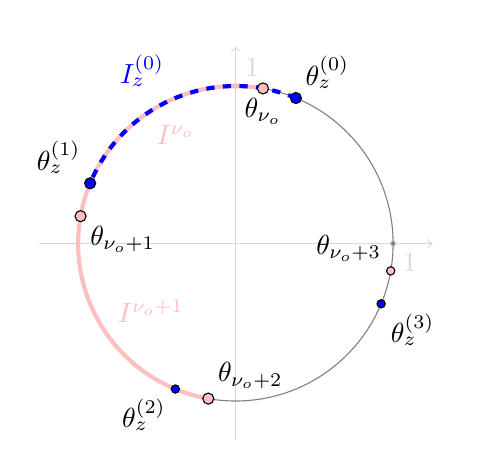
\begin{tikzpicture}
 % coordinate system
  \draw[gray!30,->] (-2.5,0) -- (2.5,0) node[right] {$\re$};
  \draw[gray!30,->] (0,-2.5) -- (0,2.5) node[above] {$\im$};
  \draw[gray!30,fill=gray] (2,0) circle (1pt) node[below right] {1};
  \draw[gray!30,fill=gray] (0,2) circle (1pt) node[above right] {1};

    \draw[gray] (0,0) circle (2cm);
    
   \draw[pink, line width=1.5pt] (80:2cm) arc (80:170:2cm) node[midway, below right] {$I^{\nu_o}$};
   \draw[pink, line width=1.5pt] (170:2cm) arc (170:260:2cm) node[midway, above right] {$I^{\nu_o+1}$};
    \draw[blue, dashed, line width=1.5pt] (67.5:2cm) arc (67.5:157.5:2.cm) node[midway, above left] {$I_z^{(0)}$};

   
    % Stokes directions for z
  \draw[fill=blue] (67.5:2cm) circle (2pt) node[above right]{$\theta_z^{(0)}$};
  \draw[fill=blue] (157.5:2cm) circle (2pt) node[above left]{$\theta_z^{(1)}$};
  \draw[fill=blue] (247.5:2cm) circle (1.5pt) node[below left]{$\theta_z^{(2)}$};
  \draw[fill=blue] (337.5:2cm) circle (1.5pt) node[below right]{$\theta_z^{(3)}$};

    %theta_\nu_o
    \draw[fill=pink] (80:2cm) circle (2pt) node[below] {$\theta_{\nu_o}$};
    \draw[fill=pink] (170:2cm) circle (2pt) node[below right] {$\theta_{\nu_o+1}$};
    \draw[fill=pink] (260:2cm) circle (2pt) node[above right] {$\theta_{\nu_o+2}$};
    \draw[fill=pink] (350:2cm) circle (1.5pt) node[above left] {$\theta_{\nu_o+3}$};
  
\end{tikzpicture}
\captionsetup{font=small}
\caption{Case 1a) with $\arg(z) = \frac{\pi}{4}$ and $\theta_{\nu_o}=\frac{4\pi}{9} \in [\frac{\pi}{4},\frac{\pi}{2})$.}
\end{minipage}
\hfill
\begin{minipage}{0.48\textwidth}
\centering
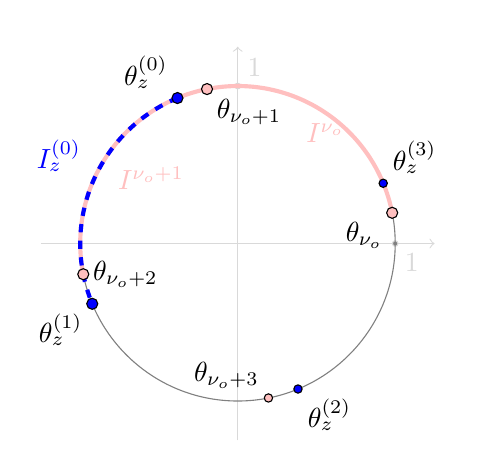
\begin{tikzpicture}
 % coordinate system
  \draw[gray!30,->] (-2.5,0) -- (2.5,0) node[right] {$\re$};
  \draw[gray!30,->] (0,-2.5) -- (0,2.5) node[above] {$\im$};
  \draw[gray!30,fill=gray] (2,0) circle (1pt) node[below right] {1};
  \draw[gray!30,fill=gray] (0,2) circle (1pt) node[above right] {1};

  \draw[gray] (0,0) circle (2cm);

   
    \draw[pink, line width=1.5pt] (11.25:2cm) arc (11.25:101.25:2cm) node[midway, below] {$I^{\nu_o}$};
    \draw[pink, line width=1.5pt] (101.25:2cm) arc (101.25:191.25:2cm) node[midway, below right] {$I^{\nu_o+1}$};
   
   \draw[blue, dashed, line width=1.5pt] (112.5:2cm) arc (112.5:202.5:2.cm) node[midway, above left] {$I_z^{(0)}$};

    % Stokes directions for z
  \draw[fill=blue] (112.5:2cm) circle (2pt) node[above left]{$\theta_z^{(0)}$};
  \draw[fill=blue] (202.5:2cm) circle (2pt) node[below left]{$\theta_z^{(1)}$};
  \draw[fill=blue] (292.5:2cm) circle (1.5pt) node[below right]{$\theta_z^{(2)}$};
  \draw[fill=blue] (22.5:2cm) circle (1.5pt) node[above right]{$\theta_z^{(3)}$};

    \draw[fill=pink] (11.25:2cm) circle (2pt) node[below left] {$\theta_{\nu_o}$};
    \draw[fill=pink] (101.25:2cm) circle (2pt) node[below right] {$\theta_{\nu_o+1}$};
    \draw[fill=pink] (191.25:2cm) circle (2pt) node[right] {$\theta_{\nu_o+2}$};
    \draw[fill=pink] (281.25:2cm) circle (1.5pt) node[above left] {$\theta_{\nu_o+3}$};
  
\end{tikzpicture}
\captionsetup{font=small}
\caption{Case 1b) with $\arg(z)=\frac{3\pi}{4}$ and $\theta_{\nu_o} = \frac{\pi}{16}\in [0, \frac{\pi}{4})$.}
\end{minipage}
\end{figure}


    \item Consider the case $\im(z) < 0$. Then with lemma (\ref{lem-nu}) we get $\theta_z^{(3)} \in \left(\frac{\pi}{4}, \frac{3\pi}{4}\right) \mod 2\pi$.
    \begin{enumerate}
            \item If $\theta_{\nu_o} \in [\frac{\pi}{4},\frac{\pi}{2}) \mod 2\pi$, then $\overline{I_z^{(3)}} \cap I^{(\nu_o)}_\epsilon \neq \varnothing$. Similar arguments as when $r$ was considered lead to $\gr_z\Lo(\overline{I_z^{(\nu+3)}}) \cong G^{(\nu_o +\nu)}_z$ for $\nu \in \Z/4\Z$. Remark that this is equivalent to $\gr_z\Lo(\overline{I_z^{(\nu)}}) \cong G^{(\nu_o+1 +\nu)}_z$ for $\nu \in \Z/4\Z$, so we get the same result as in case 1b).
            \item If $\theta_{\nu_o} \in [0,\frac{\pi}{2}) \mod 2\pi$, then $\overline{I_z^{(3)}} \cap I^{(\nu_o+1)}_\epsilon \neq \varnothing$. As before, this results in $\gr_z\Lo(\overline{I_z^{(\nu+3)}}) \cong G^{(\nu_o+ \nu+1)}_z$ for $\nu \in \Z/4\Z$. Remark that this is equivalent to $\gr_z\Lo(\overline{I_z^{(\nu)}}) \cong G^{(\nu_o +\nu)}_z$ for $\nu \in \Z/4\Z$, so we get the same result as in case 1a).
        \end{enumerate}

\begin{figure}[h!]
\begin{minipage}{0.48\textwidth}
\centering
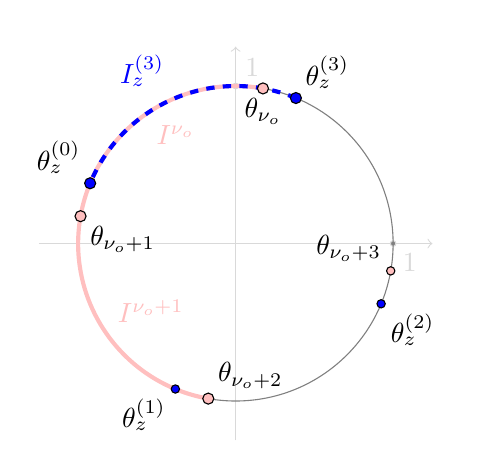
\begin{tikzpicture}
 % coordinate system
  \draw[gray!30,->] (-2.5,0) -- (2.5,0) node[right] {$\re$};
  \draw[gray!30,->] (0,-2.5) -- (0,2.5) node[above] {$\im$};
  \draw[gray!30,fill=gray] (2,0) circle (1pt) node[below right] {1};
  \draw[gray!30,fill=gray] (0,2) circle (1pt) node[above right] {1};

    \draw[gray] (0,0) circle (2cm);
    
   \draw[pink, line width=1.5pt] (80:2cm) arc (80:170:2cm) node[midway, below right] {$I^{\nu_o}$};
   \draw[pink, line width=1.5pt] (170:2cm) arc (170:260:2cm) node[midway, above right] {$I^{\nu_o+1}$};
    \draw[blue, dashed, line width=1.5pt] (67.5:2cm) arc (67.5:157.5:2.cm) node[midway, above left] {$I_z^{(3)}$};

   
    % Stokes directions for z
  \draw[fill=blue] (157.5:2cm) circle (2pt) node[above left]{$\theta_z^{(0)}$};
  \draw[fill=blue] (247.5:2cm) circle (1.5pt) node[below left]{$\theta_z^{(1)}$};
  \draw[fill=blue] (337.5:2cm) circle (1.5pt) node[below right]{$\theta_z^{(2)}$};
  \draw[fill=blue] (67.5:2cm) circle (2pt)node[above right]{$\theta_z^{(3)}$};

    %theta_\nu_o
    \draw[fill=pink] (80:2cm) circle (2pt) node[below] {$\theta_{\nu_o}$};
    \draw[fill=pink] (170:2cm) circle (2pt) node[below right] {$\theta_{\nu_o+1}$};
    \draw[fill=pink] (260:2cm) circle (2pt) node[above right] {$\theta_{\nu_o+2}$};
    \draw[fill=pink] (350:2cm) circle (1.5pt) node[above left] {$\theta_{\nu_o+3}$};
  
\end{tikzpicture}
\captionsetup{font=small}
\caption{Case 2a) with $\arg(z) = \frac{5\pi}{4}$ and $\theta_{\nu_o}=\frac{4\pi}{9} \in [\frac{\pi}{4},\frac{\pi}{2})$.}
\end{minipage}
\hfill
\begin{minipage}{0.48\textwidth}
\centering
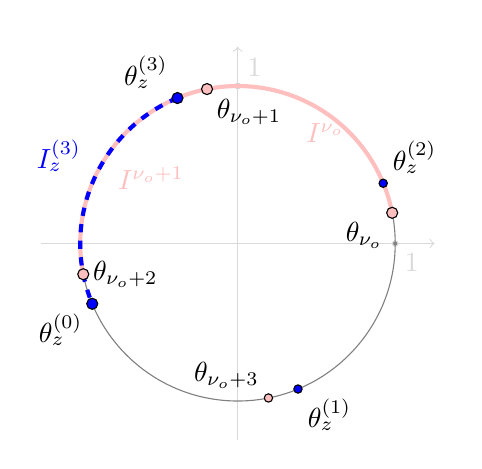
\begin{tikzpicture}
 % coordinate system
  \draw[gray!30,->] (-2.5,0) -- (2.5,0) node[right] {$\re$};
  \draw[gray!30,->] (0,-2.5) -- (0,2.5) node[above] {$\im$};
  \draw[gray!30,fill=gray] (2,0) circle (1pt) node[below right] {1};
  \draw[gray!30,fill=gray] (0,2) circle (1pt) node[above right] {1};

  \draw[gray] (0,0) circle (2cm);

   
    \draw[pink, line width=1.5pt] (11.25:2cm) arc (11.25:101.25:2cm) node[midway, below] {$I^{\nu_o}$};
    \draw[pink, line width=1.5pt] (101.25:2cm) arc (101.25:191.25:2cm) node[midway, below right] {$I^{\nu_o+1}$};
   
   \draw[blue, dashed, line width=1.5pt] (112.5:2cm) arc (112.5:202.5:2.cm) node[midway, above left] {$I_z^{(3)}$};

    % Stokes directions for z
  \draw[fill=blue] (112.5:2cm) circle (2pt) node[above left]{$\theta_z^{(3)}$};
  \draw[fill=blue] (202.5:2cm) circle (2pt) node[below left]{$\theta_z^{(0)}$};
  \draw[fill=blue] (292.5:2cm) circle (1.5pt) node[below right]{$\theta_z^{(1)}$};
  \draw[fill=blue] (22.5:2cm) circle (1.5pt) node[above right]{$\theta_z^{(2)}$};

    \draw[fill=pink] (11.25:2cm) circle (2pt) node[below left] {$\theta_{\nu_o}$};
    \draw[fill=pink] (101.25:2cm) circle (2pt) node[below right] {$\theta_{\nu_o+1}$};
    \draw[fill=pink] (191.25:2cm) circle (2pt) node[right] {$\theta_{\nu_o+2}$};
    \draw[fill=pink] (281.25:2cm) circle (1.5pt) node[above left] {$\theta_{\nu_o+3}$};
  
\end{tikzpicture}
\captionsetup{font=small}
\caption{Case 2b) with $\arg(z)=\frac{7\pi}{4}$ and $\theta_{\nu_o} = \frac{\pi}{8}\in [0, \frac{\pi}{4})$.}
\end{minipage}
\end{figure}

\end{enumerate}

This allows us to clarify $\Phi_{z}^{(\nu+1,\nu)}:\gr_z\Lo(\overline{I_z^{(\nu)}}) \to \gr_z\Lo(\overline{I_z^{(\nu+1)}})$: 

If $\gr_z\Lo(\overline{I_z^{(\nu)}}) \cong G_z^{(\nu_o+\nu)}$, then 
\[
\Phi_z^{(\nu+1,\nu)}: \gr_z\Lo(\overline{I_z^{(\nu)}}) \cong G_z^{(\nu_o+\nu)} \overset{S_{zz}^{(\nu_o+\nu+1,\nu_o+\nu)}}{\longrightarrow} G_z^{(\nu_o+\nu+1)} \cong  \gr_z\Lo(\overline{I_z^{(\nu+1)}})
\]
and similar if $\gr_z\Lo(\overline{I_z^{(\nu)}}) \cong G_z^{(\nu_o+\nu+1)}$, then 
\[
\Phi_z^{(\nu+1,\nu)}: \gr_z\Lo(\overline{I_z^{(\nu)}}) \cong G_z^{(\nu_o+\nu+1)} \overset{S_{zz}^{(\nu_o+\nu+2,\nu_o+\nu+1)}}{\longrightarrow} G_z^{(\nu_o+\nu+2)} \cong  \gr_z\Lo(\overline{I_z^{(\nu+1)}}).
\]

After having a precise description of $\mathfrak{D}(\mathfrak{L}(\sigma))$, we want to show that $\sigma$ induces a deformation datum of $\mathfrak{L}(\sigma)$ in the following.

\begin{lem}
    Let $\theta_0 \in S^1$ be generic direction with respect to $C=\{r,z\}$ with $r \in \R_{>0}$ and $z \in \C \smallsetminus \R$ and let $\sigma =((G_c^{(\nu)})_{c \in C}, S^{(\nu+1,\nu)})_{\nu \in \Z/4\Z}$ be an object in $\SD(C,\theta_0)$. Then $\sigma$ induces a deformation datum of $\mathfrak{L}(\sigma)$, that we note with $\mathfrak{R}(\sigma)$.
\end{lem}

\begin{proof} Let $\sigma = ((G_c^{(\nu)})_{c \in C}, S^{(\nu+1,\nu)})_{\nu \in \Z/4\Z}$ be an object in $\SD(C,\theta_0)$ and $\mathfrak{L}(\sigma)$ be the induced object in $\LocStgr(C)$, defined in the proof of lemma (\ref{data-to-graded}).
    As we saw in section (\ref{ShellData}), a deformation datum for a graded Stokes filtered local system $(\gr\Lo,\gr\Lo_{\leq \bullet})$ of Gaussian type $C=\{r,z\}$ with $r \in \R_{>0}$ and $z \in \C \smallsetminus \R$ can be described by 4 linear morphisms 
    \begin{multicols}{2} % Start the two-column layout
    \begin{enumerate}
        \item $\Rc_0 \coloneqq \Rc_{I_z^{(3)}}^{I_r^{(0)}}:K_{z,I_z^{(3)}} \to K_{r,I_r^{(0)}}$,
        \item $\Rc_1 \coloneqq \Rc_{I_r^{(1)}}^{I_z^{(0)}}: K_{r, I_r^{(1)}} \to K_{z,I_z^{(0)}}$,
        \item $\Rc_2 \coloneqq \Rc_{I_z^{(1)}}^{I_r^{(2)}}: K_{z,I_z^{(1)}} \to K_{r,I_r^{(2)}}$,
        \item $\Rc_3 \coloneqq \Rc_{I_r^{(3)}}^{I_z^{(2)}}: K_{r, I_r^{(3)}} \to K_{z,I_z^{(2)}}$. 
    \end{enumerate}
    \end{multicols}
    All other morphisms that appear in (\ref{Defo}) are given by the zero morphism. Since $\mathfrak{D}(\mathfrak{L}(\sigma))$ is dependant on $\im(z)$ and $\theta_0$ we have to consider different cases in order to define $(\Rc_\nu)_{\nu \in \Z/4\Z}$. Let $\nu_o \in \Z/4\Z$ be so that $\theta_{\nu_o} \in [0,\frac{\pi}{2}) \mod 2\pi$.

\begin{enumerate}
    \item First consider the case $\gr_z\Lo(\overline{I_z^{(\nu)}}) \cong G^{(\nu_o +\nu)}_z$ for $\nu \in \Z/4\Z$, so $\im(z) > 0$ and $\theta_{\nu_o} \in [\frac{\pi}{4},\frac{\pi}{2}) \mod 2\pi$ or $\im(z) <0$ and $\theta_{\nu_o} \in [0,\frac{\pi}{4}) \mod 2\pi$.
    \begin{enumerate}
        \item In the case $z \leq_{\theta_{\nu_o}} r$ the deformation datum is given by
    \begin{enumerate}
        \item $\Rc_0 \coloneqq \Rc_{I_z^{(3)}}^{I_r^{(0)}}: \gr_z\Lo(\overline{I_z^{(3)}}) \cong G_z^{(\nu_o + 3)} \overset{S_0}{\longrightarrow} G_r^{(\nu_o)} \cong \gr_r\Lo(\overline{I_r^{(0)}})$, with $S_0 \coloneqq (S_{rr}^{(\nu_o+1,\nu_o)})^{-1} \circ S_{rz}^{(\nu_o+1,\nu_o)}\circ S_{zz}^{(\nu_o,\nu_o+3)}$, 
        \item $\Rc_1 \coloneqq \Rc_{I_r^{(1)}}^{I_z^{(0)}}: \gr_r\Lo(\overline{I_r^{(1)}}) \cong G_r^{(\nu_o+1)} \overset{S_1}{\longrightarrow} G_z^{(\nu_o)} \cong \gr_z\Lo(\overline{I_z^{(0)}})$, with $S_1 \coloneqq (S_{zz}^{(\nu_o+1,\nu_o)})^{-1}\circ (S_{zz}^{(\nu_o+2,\nu_o+1)})^{-1} \circ S_{zr}^{(\nu_o+2,\nu_o+1)}$,
        \item $\Rc_2 \coloneqq \Rc_{I_z^{(1)}}^{I_r^{(2)}}: \gr_z\Lo(\overline{I_z^{(1)}}) \cong G_z^{(\nu_o+1)} \overset{S_2}{\longrightarrow} G_r^{(\nu_o+2)} \cong \gr_r\Lo(\overline{I_r^{(2)}})$, with $S_2 \coloneqq (S_{rr}^{(\nu_o+3,\nu_o+2)})^{-1} \circ S_{rz}^{(\nu_o+3,\nu_o+2)}\circ S_{zz}^{(\nu_o+2,\nu_o+1)}$ and 
        \item $\Rc_3 \coloneqq \Rc_{I_r^{(3)}}^{I_z^{(2)}}: \gr_r\Lo(\overline{I_r^{(3)}}) \cong G_r^{(\nu_o+3)} \overset{S_3}{\longrightarrow} G_z^{(\nu_o+2)} \cong \gr_z\Lo(\overline{I_z^{(2)}})$, with $S_3 \coloneqq (S_{zz}^{(\nu_o+3,\nu_o+2)})^{-1}\circ (S_{zz}^{(\nu_o,\nu_o+3)})^{-1} \circ S_{zr}^{(\nu_o,\nu_o+3)}$.
\end{enumerate}
\item Considering the case $r \leq_{\theta_{\nu_o}} z$ we get the following deformation datum:
\begin{enumerate}
        \item $\Rc_0 \coloneqq \Rc_{I_z^{(3)}}^{I_r^{(0)}}: \gr_z\Lo(\overline{I_z^{(3)}}) \cong G_z^{(\nu_o + 3)} \overset{S_0}{\longrightarrow} G_r^{(\nu_o)} \cong \gr_r\Lo(\overline{I_r^{(0)}})$, with $S_0 \coloneqq S_{rz}^{(\nu_o,\nu_o+3)}$, 
        \item $\Rc_1 \coloneqq \Rc_{I_r^{(1)}}^{I_z^{(0)}}: \gr_r\Lo(\overline{I_r^{(1)}}) \cong G_r^{(\nu_o+1)} \overset{S_1}{\longrightarrow} G_z^{(\nu_o)} \cong \gr_z\Lo(\overline{I_z^{(0)}})$, with $S_1 \coloneqq (S_{zz}^{(\nu_o+1,\nu_o)})^{-1}\circ S_{zr}^{(\nu_o+1,\nu_o)} \circ (S_{rr}^{(\nu_o+1,\nu_o)})^{-1}$,
        \item $\Rc_2 \coloneqq \Rc_{I_z^{(1)}}^{I_r^{(2)}}: \gr_z\Lo(\overline{I_z^{(1)}}) \cong G_z^{(\nu_o+1)} \overset{S_2}{\longrightarrow} G_r^{(\nu_o+2)} \cong \gr_r\Lo(\overline{I_r^{(2)}})$, with $S_2 \coloneqq  S_{rz}^{(\nu_o+2,\nu_o+1)}$ and 
        \item $\Rc_3 \coloneqq \Rc_{I_r^{(3)}}^{I_z^{(2)}}: \gr_r\Lo(\overline{I_r^{(3)}}) \cong G_r^{(\nu_o+3)} \overset{S_3}{\longrightarrow} G_z^{(\nu_o+2)} \cong \gr_z\Lo(\overline{I_z^{(2)}})$, with $S_3 \coloneqq (S_{zz}^{(\nu_o+3,\nu_o+2)})^{-1}\circ S_{zr}^{(\nu_o+3,\nu_o+2)} \circ (S_{rr}^{(\nu_o+3,\nu_o+2)})^{-1}$.
\end{enumerate}
\end{enumerate}


\item Now consider the case $\gr_z\Lo(\overline{I_z^{(\nu)}}) \cong G^{(\nu_o+1+\nu)}_z$ for $\nu \in \Z/4\Z$, so $\im(z) > 0$ and $\theta_{\nu_o} \in [0,\frac{\pi}{4}) \mod 2\pi$ or $\im(z) <0$ and $\theta_{\nu_o} \in [\frac{\pi}{4},\frac{\pi}{2}) \mod 2\pi$.
\begin{enumerate}
    \item In the case $z \leq_{\theta_{\nu_o}} r$ we get
    \begin{enumerate}
        \item $\Rc_0 \coloneqq \Rc_{I_z^{(3)}}^{I_r^{(0)}}: \gr_z\Lo(\overline{I_z^{(3)}}) \cong G_z^{(\nu_o)} \overset{S_0}{\longrightarrow} G_r^{(\nu_o)} \cong \gr_r\Lo(\overline{I_r^{(0)}})$ with $S_0 \coloneqq (S_{rr}^{(\nu_o+1,\nu_o)})^{-1} \circ S_{rz}^{(\nu_o+1,\nu_o)}$,
        \item $\Rc_1 \coloneqq \Rc_{I_r^{(1)}}^{I_z^{(0)}}: \gr_r\Lo(\overline{I_r^{(1)}}) \cong G_r^{(\nu_o+1)} \overset{S_1}{\longrightarrow} G_z^{(\nu_o+1)} \cong \gr_z\Lo(\overline{I_z^{(0)}})$, with $S_1 \coloneqq (S_{zz}^{(\nu_o+2,\nu_o+1)})^{-1} \circ S_{zr}^{(\nu_o+2, \nu_o+1)}$ 
        \item $\Rc_2 \coloneqq \Rc_{I_z^{(1)}}^{I_r^{(2)}}: \gr_z\Lo(\overline{I_z^{(1)}}) \cong G_z^{(\nu_o+2)} \overset{S_2}{\longrightarrow} G_r^{(\nu_o+2)} \cong \gr_r\Lo(\overline{I_r^{(2)}})$ with $S_2 \coloneqq (S_{rr}^{(\nu_o+3,\nu_o+2)})^{-1} \circ S_{rz}^{(\nu_o+3,\nu_o+2)}$ and
        \item $\Rc_3 \coloneqq \Rc_{I_r^{(3)}}^{I_z^{(2)}}: \gr_r\Lo(\overline{I_r^{(3)}}) \cong G_r^{(\nu_o+3)} \overset{S_3}{\longrightarrow} G_z^{(\nu_o+3)} \cong \gr_z\Lo(\overline{I_z^{(2)}})$ with $S_3 \coloneqq (S_{zz}^{(\nu_o,\nu_o+3)})^{-1} \circ S_{zr}^{(\nu_o, \nu_o+3)}$.
\end{enumerate}
 \item Considering the case $r \leq_{\theta_{\nu_o}} z$ we get
\begin{enumerate}
        \item $\Rc_0 \coloneqq \Rc_{I_z^{(3)}}^{I_r^{(0)}}: \gr_z\Lo(\overline{I_z^{(3)}}) \cong G_z^{(\nu_o)} \overset{S_0}{\longrightarrow} G_r^{(\nu_o)} \cong \gr_r\Lo(\overline{I_r^{(0)}})$ with $S_0 \coloneqq S_{rz}^{(\nu_o,\nu_o+3)} \circ (S_{zz}^{(\nu_o,\nu_o+3)})^{-1}$,
        \item $\Rc_1 \coloneqq \Rc_{I_r^{(1)}}^{I_z^{(0)}}: \gr_r\Lo(\overline{I_r^{(1)}}) \cong G_r^{(\nu_o+1)} \overset{S_1}{\longrightarrow} G_z^{(\nu_o+1)} \cong \gr_z\Lo(\overline{I_z^{(0)}})$, with $S_1 \coloneqq S_{zr}^{(\nu_o+1, \nu_o)} \circ (S_{rr}^{(\nu_o+1,\nu_o)})^{-1}$ 
        \item $\Rc_2 \coloneqq \Rc_{I_z^{(1)}}^{I_r^{(2)}}: \gr_z\Lo(\overline{I_z^{(1)}}) \cong G_z^{(\nu_o+2)} \overset{S_2}{\longrightarrow} G_r^{(\nu_o+2)} \cong \gr_r\Lo(\overline{I_r^{(2)}})$ with $S_2 \coloneqq S_{rz}^{(\nu_o+2,\nu_o+1)} \circ (S_{zz}^{(\nu_o+2,\nu_o+1)})^{-1}$ and
        \item $\Rc_3 \coloneqq \Rc_{I_r^{(3)}}^{I_z^{(2)}}: \gr_r\Lo(\overline{I_r^{(3)}}) \cong G_r^{(\nu_o+3)} \overset{S_3}{\longrightarrow} G_z^{(\nu_o+3)} \cong \gr_z\Lo(\overline{I_z^{(2)}})$ with $S_3 \coloneqq S_{zr}^{(\nu_o+3, \nu_o+2)} \circ (S_{rr}^{(\nu_o+3,\nu_o+2)})^{-1}$.
\end{enumerate}
\end{enumerate}
\end{enumerate}

We define $\mathfrak{R}(\sigma) \coloneqq (\Rc_\nu)_{\nu \in \Z/4\Z}$ to be the induced deformation datum of $\mathfrak{L}(\sigma)$.
\end{proof}

Next we show that $\sigma \mapsto (\mathfrak{L}(\sigma), \mathfrak{R}(\sigma))$ extends to a functor.

\begin{prop}\label{G-Funktor}
    Consider $C=\{r,z\}$ with $r \in \R_{>0}$ and $z \in \C\smallsetminus \R$ and let $\theta_0 \in S^1$ be a generic direction with respect to $C$. Define 
    \[
    \begin{matrix}
        G_{\theta_0}: & \SD(C,\theta_0) &\longrightarrow &\SH(C) \\
        & \sigma = ((G_c^{(\nu)})_{c \in C}, S^{(\nu+1,\nu)})_{\nu \in \Z/4\Z} & \longmapsto & G_{\theta_0}(\sigma)
    \end{matrix}
    \]
    where $G_{\theta_0}(\sigma) \coloneqq (\mathfrak{L}(\sigma), \mathfrak{R}(\sigma))$. Then $G_{\theta_0}$ is a functor between $\SD(C,\theta_0)$ and $\SH(C)$.
\end{prop}
\begin{proof}
    We already saw, that $G_{\theta_0}(\sigma)$ is an object in $\SH(C)$, as $\mathfrak{L}(\sigma)$ is a graded Stokes filtered local system and $\mathfrak{R}(\sigma)$ is a deformation datum of $\mathfrak{L}(\sigma)$. \\
    Now we define $G_{\theta_0}$ for morphisms in $\SD(C,\theta_0)$. Let $\lambda \in \Hom_{\SD(C,\theta_0)}(\sigma, \tilde{\sigma})$ with the Stokes data $\sigma = ((G_c^{(\nu)})_{c \in C}, S^{(\nu+1,\nu)})_{\nu \in \Z/4\Z}$, $\tilde{\sigma} = ((\tilde{G}_c^{(\nu)})_{c \in C}, \tilde{S}^{(\nu+1,\nu)})_{\nu \in \Z/4\Z}$ and the induced graded Stokes filtered local systems $\mathfrak{L}(\sigma) = (\gr\Lo, \gr\Lo_{\leq \bullet})$ and $\mathfrak{L}(\tilde{\sigma})=(\gr\tilde{\Lo}, \gr\tilde{\Lo}_{\leq \bullet})$. Then $\lambda = (\lambda^{(\nu)}:G_r^{(\nu)} \oplus G_z^{(\nu)} \to \tilde{G}_r^{(\nu)} \oplus \tilde{G}_z^{(\nu)})_{\nu \in \Z/4\Z}$ is given by
    \[
    \lambda^{(\nu)} = 
    \begin{pmatrix}
        \lambda_{r,r}^{(\nu)} & 0 \\
        0 & \lambda_{z,z}^{(\nu)} \end{pmatrix}
        :G_{r}^{(\nu)}\oplus G_z^{(\nu)} \longrightarrow \tilde{G}_{r}^{(\nu)} \oplus \tilde{G}_z^{(\nu)}.
    \]
    We will define $\phi_c: \gr_c\Lo \to \gr_c\tilde{\Lo}$ for $c \in C$ which gives us a graded morphism of local systems $G_{\theta_0}(\lambda):\gr\Lo \to \gr\tilde{\Lo}$ with $G_{\theta_0}(\lambda)(\gr\Lo_{\leq c}) \subseteq \gr\tilde{\Lo}_{\leq c}$, i.e.\ a morphism in $\Hom_{\LocStgr(C)}(\mathfrak{L}(\sigma), \mathfrak{L}(\tilde{\sigma}))$. Then it is left to check that $G_{\theta_0}(\lambda)$ is compatible with the deformation datum $\mathfrak{R}(\sigma)$ and $\mathfrak{R}(\tilde{\sigma})$.

    Since $\mathcal{B}\coloneqq \{U=(\eta_0,\eta_1) \subseteq \R/2\pi\Z \mid 0 \leq \eta_0 - \eta_1 \mod 2\pi < \frac{\pi}{2}\}$ is a basis for the topology of $S^1$,
    it is enough to define $\phi_c$ for open sets $U \in \mathcal{B}$. Recall that in the proof of (\ref{data-to-graded}) we gave a construction for $\gr_c\Lo$ that is 
    \[
    \gr_c\Lo(U) = \left\{(s_\nu)\in\prod_{\nu\in \/4\Z} \underline{G_c^{(\nu)}}_{I^{(\nu)}_\epsilon}(U \cap I^{(\nu)}_\epsilon) ~\Big\vert ~ S_{cc}^{(\nu+1, \nu)}(s_{\nu\vert_{W}}) = s_{\nu+1\vert_{W}} ~\forall \nu \in \Z/4\Z \right\}.
    \]
    Here, $(I^{(\nu)}_\epsilon)_{\nu \in \Z/4\Z}$ is a covering of open intervals with length $\frac{\pi}{2}+2\epsilon$ of $S^1$ with $0< \epsilon < \frac{\pi}{4}$ as in the proof of lemma (\ref{data-to-graded}) and $W \coloneqq U \cap I_\epsilon^{(\nu)} \cap I_{\epsilon}^{(\nu+1)}$.
    Remark that $U\cap I^{(\nu)}_\epsilon$ is connected for each $U \in \mathcal{B}$ and $\nu \in \Z/4\Z$, so $\underline{G_c^{(\nu)}}_{I^{(\nu)}_\epsilon}(U \cap I^{(\nu)}_\epsilon)$ is equal to $G_c^{(\nu)}$ if $U \cap I^{(\nu)}_\epsilon \neq \varnothing$ and equal to $0$ if not. We set
    \[
    \begin{matrix}
        \phi_c(U): &\gr_c\Lo(U) &\longrightarrow &\gr_c\tilde{\Lo}(U). \\
        & (s_\nu)_{\nu \in \Z/4\Z} & \longmapsto & (\lambda^{(\nu)}_{c,c}(s_\nu))_{\nu \in \Z/4\Z}
    \end{matrix}
    \]
    As $\lambda_{c,c}^{(\nu)}(s_\nu) \in \tilde{G}_c^{(\nu)}$ and $\tilde{S}_{cc}^{(\nu+1,\nu)}(\lambda_{c,c}^{(\nu)}(s_\nu)) = \lambda_{c,c}^{(\nu+1)}(S^{(\nu+1,\nu)}_{cc}(s_\nu)) = \lambda_{c,c}^{(\nu+1)}(s_{\nu+1})$, the morphism $\phi_c(U)$ is well-defined. Since $\phi_c$ commutes with the restriction morphisms of the sheaves $\gr\Lo$ and $\gr\tilde{\Lo}$, $\phi_c$ is a morphism of local systems. Given that $\gr\Lo$ is the direct sum of $\gr_r\Lo$ and $\gr_z\Lo$ and similarly $\gr\tilde{\Lo} = \gr_r\tilde{\Lo} \oplus \gr_z\tilde{\Lo}$, it is straightforward to define $G_{\theta_0}(\lambda) \in \Hom_{\Loc_{S^1}}(\gr\Lo,\gr\tilde{\Lo}):$
    When we decompose $G_{\theta_0}(\lambda)$ into blocks of morphisms of local systems \[(\phi_{ji}: \gr_{c_i}\Lo \to \gr_{c_j}\tilde{\Lo})_{c_i,c_j\in \{r,z\}}\] we have $\phi_{ji} = 0$ if $c_i \neq c_j$ and $\phi_{ji} = \phi_{c_i}$ if $c_i =c_j$.
    
    We have to show that $G_{\theta_0}(\lambda)(\gr\Lo_{\leq c}) \subseteq \gr\tilde{\Lo}_{\leq c}$ for all $c \in \C$ which can be checked on the stalks, namely $G_{\theta_0}(\lambda)(\gr\Lo_{\leq c})_\theta \subseteq \gr\tilde{\Lo}_{\leq c,\theta}$ for all $c \in \C$ and $\theta \in S^1$. For any $c \in \C$ and $\theta \in S^1$ we have
    \[
    (\gr\Lo_{\leq c})_\theta = \bigoplus_{c' \in C} \beta_{c' \leq c}(\gr_{c'}\Lo)_\theta = \bigoplus_{c' \leq_\theta c} \gr_{c'}\Lo_\theta
    \]
    and similarly $\gr\tilde{\Lo}_{\leq c,\theta} = \bigoplus_{c' \leq_\theta c} \gr_{c'}\tilde{\Lo}_\theta$. 
    Given that $\phi_c(\gr_c\Lo_{\theta}) \subseteq \gr_c\tilde{\Lo}_{\theta}$ for $c \in C$, it follows that $G_{\theta_0}(\lambda)(\gr\Lo_{\leq c})_\theta \subseteq \gr\tilde{\Lo}_{\leq c,\theta}$. Thus $G_{\theta_0}(\lambda) \in \Hom_{\LocStgr(C)}(\mathfrak{L}(\sigma),\mathfrak{L}(\tilde{\sigma}))$.

    ~\newline
    To see that $G_{\theta_0}(\lambda)$ is a morphism of Stokes shells, it is left to check that it is compatible with the deformation datum $\mathfrak{R}(\sigma)=(\Rc_\nu)_{\nu \in \Z/4\Z}$ and $\mathfrak{R}(\tilde{\sigma})=(\tilde{\Rc}_\nu)_{\nu \in \Z/4\Z}$, i.e.\ that $G_{\theta_0}(\lambda) \circ \Rc_{\nu} = \tilde{\Rc}_{\nu} \circ G_{\theta_0}(\lambda) $ for each $\nu \in \Z/4\Z.$ As we have seen before, the deformation datum depends on $z$ and $\theta_0$, so we have to investigate different cases. Again, let $\nu_o \in \Z/4\Z$ be such that $\theta_{\nu_o} = \theta_0+\nu_o\frac{\pi}{2} \in [0, \frac{\pi}{2}) \mod 2\pi.$
    
   We only consider the case $\im(z)>0$ and $\theta_{\nu_o} \in [\frac{\pi}{4},\frac{\pi}{2}) \mod 2\pi$ (resp.\ $\im(z)<0$ and $\theta_{\nu_o} \in [0,\frac{\pi}{4})\mod 2\pi$), because all other cases can be proven analogously. Thus, in our scenario, we have $\gr_c\Lo(\overline{I_c^{(\nu)}}) \cong G^{(\nu_o +\nu)}_c$ and $\gr_c\tilde{\Lo}(\overline{I_c^{(\nu)}}) \cong \tilde{G}^{(\nu_o +\nu)}_c$ for $\nu \in \Z/4\Z$, $c \in C$. 
   We denote these isomorphisms by \[\psi_c^{(\nu)}: \gr_c\Lo(\overline{I_c^{(\nu)}}) \to G_c^{(\nu_o+\nu)}.\] In particular, $\psi_c^{(\nu)}$ maps a tuple $(s_\nu)_{\nu \in \Z/4\Z} \in \gr_c\Lo(\overline{I_c^{(\nu)}})$ to $s_{\nu_o+\nu} \in G_c^{(\nu_o+\nu)}$. Analogously we define $\tilde{\psi}_c^{(\nu)}: \gr_c\tilde{\Lo}(\overline{I_c^{(\nu)}}) \to \tilde{G}_c^{(\nu_o+\nu)}$.

        In the case $z \leq_{\theta_{\nu_o}} r$ the deformation datum $\mathfrak{R}(\sigma)$ is given by
        \begin{align*}
        \Rc_k: &\gr_z\Lo(\overline{I_z^{(k+3)}}) \cong G_z^{(\nu_o + k + 3)} \overset{S_k}{\longrightarrow} G_r^{(\nu_o+k)} \cong \gr_r\Lo(\overline{I_r^{(k)}}) \text{ with } \\
        &S_k \coloneqq (S_{rr}^{(\nu_o+k+1,\nu_o+k)})^{-1} \circ S_{rz}^{(\nu_o+k+1,\nu_o+k)}\circ S_{zz}^{(\nu_o+k,\nu_o+k+3)} \text{ for } k \in \{0,2\} \\
        \Rc_k: &\gr_r\Lo(\overline{I_r^{(k)}}) \cong G_r^{(\nu_o+k)} \overset{S_k}{\longrightarrow} G_z^{(\nu_o+k+3)} \cong \gr_z\Lo(\overline{I_z^{(k+3)}}) \text{ with } \\
        & S_k \coloneqq (S_{zz}^{(\nu_o+k,\nu_o+k+3)})^{-1}\circ (S_{zz}^{(\nu_o+k+1,\nu_o+k)})^{-1} \circ S_{zr}^{(\nu_o+k+1,\nu_o+k)} \text{ for } k \in \{1,3\}
        \end{align*}
        and the same holds for $\tilde{\Rc}_k$.

        As for each interval $I \in \{I_c^{(\nu)} \mid c \in C, \nu \in \Z/4\Z\}$ we have  \[ 
        \begin{matrix}    
             G_{\theta_0}(\lambda)(\overline{I_c^{(\nu)}})_{\vert\gr_c\Lo(\overline{I_c^{(\nu)}})}= \phi_c(\overline{I_c^{(\nu)}}):&\gr_c\Lo(\overline{I_c^{(\nu)}}) &\to &\gr_c\tilde{\Lo}(\overline{I_c^{(\nu)}}),
             \\ &(s_\nu)_{\nu \in \Z/4\Z} &\mapsto & (\lambda_{c,c}^{(\nu)}(s_\nu))_{\nu \in \Z/4\Z}
        \end{matrix}\] we have to prove that for $k \in \{0,2\}$ the diagram 

    \begin{center}
        \begin{tikzcd}[row sep=1.5cm, column sep=2cm]
         & \gr_z\Lo(\overline{I_z^{(k+3)}}) \arrow[d, swap,"\Rc_k"] \arrow[r, "\phi_z(\overline{I_z^{(k+3)}})"] & \gr_z\tilde{\Lo}(\overline{I_z^{(k+3)}}) \arrow[d, "\tilde{\Rc}_k"]&\\
        & \gr_r\Lo(\overline{I_r^{(k)}}) \arrow[r, swap, "\phi_r(\overline{I_r^{(k)}})"] &  \gr_r\tilde{\Lo}(\overline{I_r^{(k)}})&
        \end{tikzcd}
    \end{center}
        
        is commutative. 
        This holds as $\lambda^{(k+1)}S^{(k+1,k)} = \tilde{S}^{(k+1,k)}\lambda^{(k)}$. More precisely, by definition of $\phi_c$ for $c \in C, \nu \in \Z/4\Z$ \[ \tilde{\psi}_c^{(\nu)}\phi_c(\overline{I_c^{(\nu)}}) =\lambda_{c,c}^{(\nu_o+\nu)}\psi_c^{(\nu)}\] holds. Thus for $k \in \{0,2\}$
        \begin{align*} 
        \tilde{\Rc}_k \circ \phi_z(\overline{I_z^{(k+3)}}) &= (\tilde{\psi}_r^{(k)})^{-1}\tilde{S}_k\tilde{\psi}_z^{(k+3)}\phi_z(\overline{I_z^{(k+3)}})=(\tilde{\psi}_r^{(k)})^{-1}\tilde{S}_k\lambda_{z,z}^{(\nu_o+k+3)}\psi_z^{(k+3)}  \\ &= (\tilde{\psi}_r^{(k)})^{-1}\lambda_{r,r}^{(\nu_o+k)}S_k\psi_z^{(k+3)} = \phi_r(\overline{I_r^{(k)}})(\psi_r^{(k)})^{-1}S_k\psi_z^{(k+3)} \\
        & = \phi_r(\overline{I_r^{(k)}})\circ \Rc_k.
        \end{align*}

        Similarly for $k \in \{1,3\}$ one can show that the following diagram commutes:

        \begin{center}
        \begin{tikzcd}[row sep=1.5cm, column sep=2cm]
         & \gr_r\Lo(\overline{I_r^{(k)}}) \arrow[d, swap,"\Rc_k"] \arrow[r, "\phi_r(\overline{I_r^{(k)}})"] & \gr_r\tilde{\Lo}(\overline{I_r^{(k)}}) \arrow[d, "\tilde{\Rc}_k"]&\\
        & \gr_z\Lo(\overline{I_z^{(k+3)}}) \arrow[r, swap, "\phi_z(\overline{I_z^{(k+3)}})"] &  \gr_z\tilde{\Lo}(\overline{I_z^{(k+3)}})&
        \end{tikzcd}
    \end{center}
    
    
        
    Thus $G_{\theta_0}(\lambda)$ is compatible with the deformation datum $\mathfrak{R}(\sigma)$ and $\mathfrak{R}(\tilde{\sigma})$ and finally $G_{\theta_0}(\lambda) \in \Hom_{\SH(C)}(\StSh,\tilde{\StSh})$. 
    The case $r \leq_{\theta_{\nu_o}} z$ can be proven analogously.
    
    By the definition of $G_{\theta_0}$ on morphisms of $\SD(C,\theta_0)$, the functoriality of $G_{\theta_0}$ follows immediately.  
\end{proof}


\section{Equivalence of categories: $\SD(C,\theta_0)$ and $\SH(C)$}

After constructing the functors $F_{\theta_0}$ and $G_{\theta_0}$ we finally want to show that these are  equivalences of categories. Without loss of generality we assume $\theta_0 \in [0,\frac{\pi}{2})$.

\begin{thm} Let $\theta_0 \in [0,\frac{\pi}{2})$ be a generic direction with respect to $C =\{r,z\}$ with $r \in \R_{>0}$ and $z \in \C\smallsetminus \R$. Then $G_{\theta_0}$ (defined in \ref{G-Funktor}) is a quasi-inverse functor of $F_{\theta_0}$ (defined in \ref{F-functor}).
\end{thm}


\begin{proof}
We first check $F_{\theta_0} \circ G_{\theta_0} \cong \id_{\SD(C,\theta_0)}$. Let $\sigma = ((G_c^{(\nu)})_{c \in C}, S^{(\nu+1,\nu)})_{\nu \in \Z/4\Z}$ be an object in $\SD(C,\theta_0)$ and $G_{\theta_0}(\sigma) = ( \mathfrak{L}(\sigma), \mathfrak{R}(\sigma))$ the associated Stokes shell. We solely consider $\im(z) >0$, $\theta_0 \in [\frac{\pi}{4}, \frac{\pi}{2})$ (resp.\ $\im(z) <0$ and $\theta_0 \in [0, \frac{\pi}{4})$) and $z\leq_{\theta_0}r$ as all other cases can be proven similar. In this scenario we already saw that $\gr_c\Lo(\overline{I_c^{(\nu)}}) \cong G_c^{(\nu)}$ for each $\nu \in \Z/4\Z$ and $c\in C$. As in the proof of (\ref{G-Funktor}), we label this isomorphism by $\psi_c^{(\nu)} : \gr_c\Lo(\overline{I_c^{(\nu)}}) \longrightarrow G_c^{(\nu)}$. 

We get $F_{\theta_0}(G_{\theta_0}(\sigma)) = ((\tilde{G}_c^{(\nu)})_{c \in C}, \tilde{S}^{(\nu+1,\nu)})_{\nu \in \Z/4\Z}$ where 

\begin{itemize}
    \item $\tilde{G}_r^{(\nu)} = \gr_r\Lo(\overline{I_r^{(\nu)}}) \overset{\psi_r^{(\nu)}}{\cong} G_r^{(\nu)}$,
    \item $\tilde{G}_z^{(\nu)} = \gr_z\Lo(\overline{I_z^{(\nu+3)}}) \overset{\psi_z^{(\nu+3)}}{\cong} G_z^{(\nu+3)}$, 
    \item $\tilde{S}^{(\nu+1,\nu)} =
        \begin{pmatrix}
            \Phi^{(\nu,\nu+3)}_z & 0\\
             \Phi_r^{(\nu+1,\nu)} \Rc_{\nu} & \Phi_r^{(\nu+1,\nu)}
        \end{pmatrix}$ for $\nu \in \{0,2\}$ and
    \item $\tilde{S}^{(\nu+1,\nu)} = \begin{pmatrix}
            \Phi^{(\nu,\nu+3)}_z & \Phi_z^{(\nu,\nu+3)} \Rc_\nu\\
            0 & \Phi_r^{(\nu+1,\nu)}
        \end{pmatrix}$ for $\nu \in \{1,3\}$,
\end{itemize}


where $\Phi_c^{(\nu+1,\nu)}: \gr_c\Lo(\overline{I_c^{(\nu)}}) \to \gr_c\Lo(\overline{I_c^{(\nu+1)}})$ is given by $(\psi_c^{(\nu+1)})^{-1}S_{cc}^{(\nu+1,\nu)}\psi_c^{(\nu)}$ for $c \in C$ and 
\begin{itemize}
    \item for $\nu \in \{0,2\}$, $\Rc_\nu: \gr_z\Lo(\overline{I_z^{(\nu+3)}}) \longrightarrow \gr_r\Lo(\overline{I_r^{(\nu)}})$ is given by
        \[\Rc_\nu = (\psi_r^{(\nu)})^{-1}(S_{rr}^{(\nu+1,\nu)})^{-1} S_{rz}^{(\nu+1,\nu)} S_{zz}^{(\nu,\nu+3)}\psi_z^{(\nu+3)}\] and
    \item for $\nu \in \{1,3\}$, $\Rc_\nu: \gr_r\Lo(\overline{I_r^{(\nu)}}) \longrightarrow \gr_z\Lo(\overline{I_z^{(\nu+3)}})$ is given by
        \[\Rc_\nu = (\psi_z^{(\nu+3)})^{-1} (S_{zz}^{(\nu,\nu+3)})^{-1}(S_{zz}^{(\nu+1,\nu)})^{-1} S_{zr}^{(\nu+1,\nu)}\psi_r^{(\nu)}.\]
\end{itemize}
Setting
\[
\alpha_\sigma^{(\nu)} \coloneqq \begin{pmatrix}
    S_{zz}^{(\nu,\nu+3)}\psi_z^{(\nu+3)} & 0 \\
    0 & \psi_r^{(\nu)}
\end{pmatrix} : \tilde{G}_z^{(\nu)} \oplus \tilde{G}_r^{(\nu)} \to G_z^{(\nu)} \oplus G_r^{(\nu)}
\]
for $\nu \in \Z/4\Z$ gives a morphism $\alpha_\sigma \coloneqq (\alpha_{\sigma}^{(\nu)})_{\nu \in \Z/4\Z}\in \Hom_{\SD(C,\theta_0)}(F_{\theta_0}(G_{\theta_0}(\sigma)),\sigma)$ as for $\nu \in \{0,2\}$
\begin{align*}
\alpha_\sigma^{(\nu+1)}\tilde{S}^{(\nu+1,\nu)} & = \begin{pmatrix}
    S_{zz}^{(\nu+1,\nu)}\psi_z^{(\nu)} & 0 \\
    0 & \psi_r^{(\nu+1)}
\end{pmatrix} \begin{pmatrix}
            \Phi^{(\nu,\nu+3)}_z & 0\\
            \Phi_r^{(\nu+1,\nu)} \Rc_{\nu} & \Phi_r^{(\nu+1,\nu)}
        \end{pmatrix} = \\
        & =  \begin{pmatrix}
            S_{zz}^{(\nu+1,\nu)}S_{zz}^{(\nu,\nu+3)}\psi_z^{(\nu+3)} & 0 \\
            S_{rz}^{(\nu+1,\nu)} S_{zz}^{(\nu,\nu+3)}\psi_z^{(\nu+3)} & S_{rr}^{(\nu+1,\nu)}\psi_r^{(\nu)}
        \end{pmatrix} = \\
        & = \begin{pmatrix}
            S_{zz}^{(\nu+1,\nu)} & 0 \\
             S_{rz}^{(\nu+1,\nu)} & S_{rr}^{(\nu+1,\nu)}
        \end{pmatrix} \begin{pmatrix}
            S_{zz}^{(\nu,\nu+3)}\psi_z^{(\nu+3)} &  0 \\
            0& \psi_r^{(\nu)}
        \end{pmatrix} = S^{(\nu+1,\nu)}\alpha_\sigma^{(\nu)}
\end{align*}
and analogue for $\nu \in \{1,3\}$ 
\begin{align*}
\alpha_\sigma^{(\nu+1)}\tilde{S}^{(\nu+1,\nu)} & = \begin{pmatrix}
    S_{zz}^{(\nu+1,\nu)}\psi_z^{(\nu)} & 0 \\
    0 & \psi_r^{(\nu+1)}
\end{pmatrix} \begin{pmatrix}
            \Phi^{(\nu,\nu+3)}_z & \Phi_z^{(\nu,\nu+3)} \Rc_\nu\\
            0 & \Phi_r^{(\nu+1,\nu)}
        \end{pmatrix} = \\
        & = \begin{pmatrix}
            S_{zz}^{(\nu+1,\nu)}S_{zz}^{(\nu,\nu+3)}\psi_z^{(\nu+3)} & S_{zr}^{(\nu+1,\nu)}\psi_r^{(\nu)} \\
            0 & S_{rr}^{(\nu+1,\nu)}\psi_r^{(\nu)}
        \end{pmatrix} = \\
        & = \begin{pmatrix}
            S_{zz}^{(\nu+1,\nu)} & S_{rz}^{(\nu+1,\nu)} \\
             0 & S_{rr}^{(\nu+1,\nu)}
        \end{pmatrix} \begin{pmatrix}
            S_{zz}^{(\nu,\nu+3)}\psi_z^{(\nu+3)} &  0 \\
            0& \psi_r^{(\nu)}
        \end{pmatrix} = S^{(\nu+1,\nu)}\alpha_\sigma^{(\nu)}.
\end{align*}
Since $\alpha_\sigma^{(\nu)}$ is an isomorphism of vector spaces for each $\nu$, $\alpha_\sigma$ is an isomorphism in $\SD(C,\theta_0)$. Thus we have indeed $F_{\theta_0}(G_{\theta_0}(\sigma)) \cong \sigma$. It is left to show that $\alpha \coloneqq (\alpha_\sigma)_{\sigma \in \SD(C,\theta_0)}$ defines a natural transformation $F_{\theta_0}G_{\theta_0} \Rightarrow \id_{\SD(C,\theta_0)}$.

Let $\lambda \in \Hom_{\SD(C,\theta_0)}(\sigma, \tilde{\sigma})$ be a morphism between $\sigma=((G_c^{(\nu)})_{c \in C}, S^{(\nu+1,\nu)})_{\nu \in \Z/4\Z}$ to $\tilde{\sigma}=((\tilde{G}_c^{(\nu)})_{c \in C}, \tilde{S}^{(\nu+1,\nu)})_{\nu \in \Z/4\Z}$. Again we write $\lambda=(\lambda^{(\nu)})_{\nu \in \Z/4\Z}$ with \[\lambda^{(\nu)} = \begin{pmatrix}
    \lambda_{z,z}^{(\nu)} & 0 \\ 
    0 & \lambda_{r,r}^{(\nu)}
\end{pmatrix}: G_z^{(\nu)} \oplus G_r^{(\nu)} \to \tilde{G}_z^{(\nu)} \oplus \tilde{G}_r^{(\nu)}.\] Then
\[
F_{\theta_0}(G_{\theta_0}(\lambda))^{(\nu)}: \gr_z\Lo(\overline{I_z^{(\nu+3)}}) \oplus \gr_r\Lo(\overline{I_r^{(\nu)}})\to \gr_z\tilde{\Lo}(\overline{I_z^{(\nu+3)}}) \oplus \gr_r\tilde{\Lo}(\overline{I_r^{(\nu)}})
\]
is given by
\begin{align*}
F_{\theta_0}(G_{\theta_0}(\lambda))^{(\nu)} & = \begin{pmatrix}
    (G_{\theta_0}(\lambda))(\overline{I_z^{(\nu+3)}})\vert_{\gr_z\Lo(\overline{I_z^{(\nu+3)}})} & 0 \\ 
    0 & (G_{\theta_0}(\lambda))(\overline{I_r^{(\nu)}})\vert_{\gr_r\Lo(\overline{I_r^{(\nu)}})}
\end{pmatrix} \\ & = \begin{pmatrix}
    (\tilde{\psi}_z^{(\nu+3)})^{-1}\lambda_{z,z}^{(\nu+3)}\psi_z^{(\nu+3)} & 0 \\
    0 & (\tilde{\psi}_r^{(\nu)})^{-1}\lambda_{r,r}^{(\nu)}\psi_r^{(\nu)}
\end{pmatrix}. 
\end{align*}
Then 
\begin{align*}
\alpha_{\tilde{\sigma}}^{(\nu)}F_{\theta_0}(G_{\theta_0}(\lambda))^{(\nu)} & = 
\begin{pmatrix}
\tilde{S}_{zz}^{(\nu,\nu+3)}\tilde{\psi}_z^{(\nu+3)}(\tilde{\psi}_z^{(\nu+3)})^{-1}\lambda_{z,z}^{(\nu+3)}\psi_z^{(\nu+3)} & 0 \\
    0 & \tilde{\psi}_r^{(\nu)}(\tilde{\psi}_r^{(\nu)})^{-1}\lambda_{r,r}^{(\nu)}\psi_r^{(\nu)}
\end{pmatrix} 
\\
& =  
\begin{pmatrix}
    \tilde{S}_{zz}^{(\nu,\nu+3)}\lambda_{z,z}^{(\nu+3)}\psi_z^{(\nu+3)} & 0 \\
    0 & \lambda_{r,r}^{(\nu)}\psi_r^{(\nu)}
\end{pmatrix} \\
& = \begin{pmatrix}
    \lambda_{z,z}^{(\nu)}\tilde{S}_{zz}^{(\nu,\nu+3)}\psi_z^{(\nu+3)} & 0 \\
    0 & \lambda_{r,r}^{(\nu)}\psi_r^{(\nu)}
\end{pmatrix} \\ & = \begin{pmatrix}
\lambda_{z,z}^{(\nu)} & 0 \\ 0 & \lambda_{r,r}^{(\nu)} \end{pmatrix} \begin{pmatrix}
    S_{zz}^{(\nu,\nu+3)}\psi_z^{(\nu+3)} & 0 \\
    0 & \psi_r^{(\nu)}
\end{pmatrix}
= \lambda^{(\nu)}\alpha_{\sigma}^{(\nu)},
\end{align*}
which shows that $\alpha: F_{\theta_0}\circ G_{\theta_0} \Rightarrow \id_{\SD(C,\theta_0)}$ is a natural Isomorphism. Thus $F_{\theta_0} \circ G_{\theta_0} \cong \id_{\SD(C,\theta_0)}.$
~\newline

Now we check $G_{\theta_0}\circ F_{\theta_0} \cong \id_{\SH(C)}$. Let $\StSh =((\gr\Lo,\gr\Lo_{\leq \bullet}),\Defo)$ be a Stokes shell of Gaussian type $C$ and $F_{\theta_0}(\StSh) = ((G_c^{(\nu)})_{c \in C}, S^{(\nu+1,\nu)})_{\nu \in \Z/4\Z}$ the associated object in $\SD(C,\theta_0)$. Since all cases follow a similar logic, we solely proof $G_{\theta_0}\circ F_{\theta_0} \cong \id_{\SH(C)}$ for $\im(z) >0$, $\theta_0 \in [\frac{\pi}{4}, \frac{\pi}{2})$ (resp.\ $\im(z) <0$, $\theta_0 \in [0, \frac{\pi}{4})$) and $z\leq_{\theta_0}r$. First notice that by construction $\mathfrak{L}(F_{\theta_o}(\StSh))=(\gr\tilde{\Lo},\gr\tilde{\Lo}_{\leq \bullet}) \cong (\gr\Lo,\gr\Lo_{\leq \bullet})$: 

It is enough to check $\gr_c\Lo \cong \gr_c\tilde{\Lo}$ for all $c \in C$. We begin with $r \in C$. Recall that $G_r^{(\nu)} = \gr_r\Lo(\overline{I_r^{(\nu)}})$ and $\gr_r\tilde{\Lo}$ is the sheaf that one receives gluing $(\underline{G_r^{(\nu)}}_{I^{(\nu)}_\epsilon})_{\nu \in \Z/4\Z}$ via the isomorphisms $(S_{rr}^{(\nu+1,\nu)})_{\nu \in \Z/4\Z}$ of $F_{\theta_0}(\StSh)$, that are $(\Phi_r^{(\nu+1,\nu)})_{\nu \in \Z/4\Z}$ of $\mathfrak{D}(\StSh)$. 

Since $\gr_r\Lo$ is a local system, in particular constant on  the interval $I^{(\nu)}_\epsilon$ (given as in the proof of lemma (\ref{data-to-graded})) and since $\overline{I_r^{(\nu)}}$ is connected we get isomorphisms

\[
\phi_r^{(\nu)}: \gr_r\Lo_{\vert_{I^{(\nu)}_\epsilon}} \longrightarrow \underline{\gr_r\Lo(\overline{I_r^{(\nu)}})}_{I_\epsilon^{(\nu)}} = \underline{G_r^{(\nu)}}_{I^{(\nu)}_\epsilon}.
\]

As $\Phi_r^{(\nu+1,\nu)}$ is defined by $\gr_r\Lo(\overline{I_r^{(\nu)}}) \cong \gr_r\Lo_{\theta_r^{(\nu+1)}} \cong \gr_r\Lo(\overline{I_r^{(\nu+1)}})$ and since $\theta_r^{(\nu+1)} \in I_\epsilon^{(\nu)} \cup I_\epsilon^{(\nu+1)}$
the morphisms $(\phi_r^{(\nu)})_{\nu \in \Z/4\Z}$ satisfy the condition 
\[
\Phi_{r}^{(\nu+1,\nu)} = \phi_r^{(\nu+1)}\circ (\phi_r^{(\nu)})^{-1}
\]
on $I^{(\nu)}_\epsilon \cap I^{(\nu+1)}_\epsilon$. Since the glued sheaf $\gr_r\tilde{\Lo}$ is unique up to isomorphim (cf.\ lemma (\ref{gluedsheaf})), there exists an isomorphism $\lambda_r : \gr_r\Lo \to \gr_r\tilde{\Lo}$, mapping $s \in \gr\Lo(U)$ to $(\phi_r^{(\nu)}(U \cap I_\epsilon^{(\nu)})(s_{\vert_{U \cap I_\epsilon^{(\nu)}}}))_{\nu \in \Z/4\Z}$, that lets the diagram 
\begin{center}
        \begin{tikzcd}[row sep=1.5cm, column sep=2cm]
         & \gr_r\Lo \arrow[d, swap,"(\bullet)_{\vert_{I_{\epsilon}^{(\nu)}}}"] \arrow[rr, "\lambda_r"] & & \gr_r\tilde{\Lo} \arrow[d, "(\bullet)_{\vert_{I_{\epsilon}^{(\nu)}}}"]&\\
        & \gr_r\Lo_{\vert_{I_\epsilon^{(\nu)}}} \arrow[rr, swap, "(\lambda_r)_{\vert_{I_\epsilon^{(\nu)}}}"] 
        \arrow[rd, "\phi_r^{(\nu)}"] & &  \gr_r\tilde{\Lo}_{\vert_{I_\epsilon^{(\nu)}}}
        \arrow[dl, "\psi_r^{(\nu)}"]& \\ & & \underline{\gr_r\Lo(\overline{I_r^{(\nu)}})}_{I_\epsilon^{(\nu)}} & &
        \end{tikzcd}
\end{center}
commute. Here, $\psi_r^{(\nu)}$ is the isomorphism of the glued sheaf $\gr_r\tilde{\Lo}$, precisely for an open set $U \subseteq I_\epsilon^{(\nu)}$,  $\psi_r^{(\nu)}(U)$ sends a tuple $(s_\nu)_{\nu \in \Z/4\Z}$ to $s_\nu \in \underline{\gr_r\Lo(\overline{I_r^{(\nu)}})}_{I_\epsilon^{(\nu)}}$.
Analogously for $z$, recall that $G_z^{(\nu)} = \gr_z\Lo(\overline{I_z^{(\nu+3)}})$ and $\gr_r\tilde{\Lo}$ is the sheaf that one receives gluing $(\underline{G_z^{(\nu)}}_{I^{(\nu)}_\epsilon})_{\nu \in \Z/4\Z}$ via the isomorphisms $(S_{zz}^{(\nu+1,\nu)})_{\nu \in \Z/4\Z}$ of $F_{\theta_0}(\StSh)$, that are $(\Phi_z^{(\nu,\nu+3)})_{\nu \in \Z/4\Z}$ of $\mathfrak{D}(\StSh)$. Since $\gr_z\Lo$ is a local system, we get isomorphisms
\[\phi_z^{(\nu)}: \gr_z\Lo_{I_\epsilon^{(\nu)}} \to \underline{\gr_z\Lo(\overline{I_z^{(\nu+3)}})}_{I_\epsilon^{(\nu)}} = \underline{G_z^{(\nu)}}_{I_\epsilon^{(\nu)}}\]
for each $\nu \in \Z/4\Z$. As $\Phi_z^{(\nu,\nu+3)}$ is given by $\gr_z\Lo(\overline{I_z^{(\nu+3)}}) \cong \gr_z\Lo_{\theta_z^{(\nu)}} \cong \gr_z\Lo(\overline{I_z^{(\nu)}})$ and since in our case $\theta_z^{(\nu)} \in I_\epsilon^{(\nu)} \cup I_\epsilon^{(\nu+3)}$ the morphisms $(\phi_z^{(\nu)})_{\nu \in \Z/4\Z}$ satisfy the equation $\Phi_z^{(\nu,\nu+3)} = \phi_z^{(\nu+1)}\phi_z^{(\nu)-1}$ on $I_\epsilon^{(\nu)} \cap I_\epsilon^{(\nu+1)}$. Again we get a commutative diagram 

\begin{center}
        \begin{tikzcd}[row sep=1.5cm, column sep=2cm]
         & \gr_z\Lo \arrow[d, swap,"(\bullet)_{\vert_{I_{\epsilon}^{(\nu)}}}"] \arrow[rr, "\lambda_z"] & & \gr_z\tilde{\Lo} \arrow[d, "(\bullet)_{\vert_{I_{\epsilon}^{(\nu)}}}"]&\\
        & \gr_z\Lo_{\vert_{I_\epsilon^{(\nu)}}} \arrow[rr, swap, "(\lambda_z)_{\vert_{I_\epsilon^{(\nu)}}}"] 
        \arrow[rd, "\phi_z^{(\nu)}"] & &  \gr_z\tilde{\Lo}_{\vert_{I_\epsilon^{(\nu)}}}
        \arrow[dl, "\psi_z^{(\nu)}"]& \\ & & \underline{\gr_z\Lo(\overline{I_z^{(\nu+3)}})}_{I_\epsilon^{(\nu)}} & &
        \end{tikzcd}
\end{center}
  The morphisms $\lambda_r,\lambda_z$ induce an isomorphism of graded Stokes filtered local systems $\beta_{\StSh}: \gr\Lo \to \gr\tilde{\Lo}$ (compare to proof of proposition (\ref{G-Funktor})). It is left to show that $\beta_{\StSh}$ is compatible with the deformation datum. To do so, we first have to describe the deformation datum of $G_{\theta_0}(F_{\theta_0}(\StSh))$. In the case we are considering ($\im(z) >0, \theta_0 \in [\frac{\pi}{4}, \frac{\pi}{2})$ and $z \leq_{\theta_0} r$), the deformation datum $\mathfrak{R}(F_{\theta_0}(\StSh))=(\tilde{\Rc}_\nu)_{\nu \in \Z/4\Z}$ is given by
\begin{align*}
        \tilde{\Rc}_\nu: &\gr_z\tilde{\Lo}(\overline{I_z^{(\nu+3)}}) \cong G_z^{(\nu + 3)} \overset{S_\nu}{\longrightarrow} G_r^{(\nu)} \cong \gr_r\tilde{\Lo}(\overline{I_r^{(\nu)}}) \text{ with } \\
        &S_\nu \coloneqq (S_{rr}^{(\nu+1,\nu)})^{-1} \circ S_{rz}^{(\nu+1,\nu)}\circ S_{zz}^{(\nu,\nu+3)} \text{ for } \nu \in \{0,2\}, \\
        \tilde{\Rc}_\nu: &\gr_r\tilde{\Lo}(\overline{I_r^{(\nu)}}) \cong G_r^{(\nu)} \overset{S_\nu}{\longrightarrow} G_z^{(\nu+3)} \cong \gr_z\tilde{\Lo}(\overline{I_z^{(\nu+3)}}) \text{ with } \\
        & S_\nu \coloneqq (S_{zz}^{(\nu,\nu+3)})^{-1}\circ (S_{zz}^{(\nu+1,\nu)})^{-1} \circ S_{zr}^{(\nu+1,\nu)} \text{ for } \nu \in \{1,3\},
\end{align*}

where 
\begin{align*}
    S^{(\nu+1,\nu)} & = \begin{pmatrix}
        \Phi_z^{(\nu,\nu+3)} & 0 \\
        \Phi_r^{(\nu+1,\nu)} \circ \Rc_\nu & \Phi_r^{(\nu+1,\nu)} 
    \end{pmatrix} &\text{ for } \nu \in \{0,2\} \text{ and} \\
    S^{(\nu+1,\nu)} & = \begin{pmatrix}
        \Phi_z^{(\nu,\nu+3)} & \Phi_z^{(\nu,\nu+3)} \circ \Rc_\nu \\
        0 & \Phi_r^{(\nu+1,\nu)} 
    \end{pmatrix} &\text{ for } \nu \in \{1,3\}.
\end{align*}

Thus the deformation datum $(\tilde{\Rc}_\nu)_{\nu \in \Z/4\Z}$ simplifies to 

\begin{align*}
        \tilde{\Rc}_\nu: &\gr_z\tilde{\Lo}(\overline{I_z^{(\nu+3)}}) \overset{\psi_z^{(\nu+3)}}{\cong} G_z^{(\nu + 3)} \overset{S_\nu}{\longrightarrow} G_r^{(\nu)} \overset{\psi_r^{(\nu)}}{\cong} \gr_r\tilde{\Lo}(\overline{I_r^{(\nu)}}) \text{ with } \\
        &S_\nu \coloneqq \Rc_\nu \circ \Phi_{z}^{(\nu+3, \nu+2)} \text{ for } \nu \in \{0,2\}, \\
        \tilde{\Rc}_\nu: &\gr_r\tilde{\Lo}(\overline{I_r^{(\nu)}}) \overset{\psi_r^{(\nu)}}{\cong} G_r^{(\nu)} \overset{S_\nu}{\longrightarrow} G_z^{(\nu+3)} \overset{\psi_z^{(\nu+3)}}{\cong} \gr_z\tilde{\Lo}(\overline{I_z^{(\nu+3)}}) \text{ with } \\
        & S_\nu \coloneqq (\Phi_z^{(\nu+3,\nu+2)})^{-1} \circ \Rc_\nu \text{ for } \nu \in \{1,3\}.
\end{align*}

The proof that $\beta_{\StSh}$ is compatible with the deformation datum can be done analogously to the proof of (\ref{G-Funktor}). Therefore we consider $\beta_{\StSh\vert \gr_c\Lo}= \lambda_c : \gr_c\Lo \to \gr_c\tilde{\Lo}$ for $c \in \{r,z\}$ and for $\nu \in \{0,2\}$ one has to check that 
\[\lambda_r(\overline{I_r^{(\nu)}}) \circ \Rc_\nu = \tilde{\Rc}_\nu \circ \lambda_z(\overline{I_z^{(\nu+3)}}),\]

which follows directly by the definition of $\tilde{\Rc}_\nu$ and the gluing data $\phi_r^{(\nu)}, \phi_z^{(\nu+3)}$. Since $\lambda_r,\lambda_z$ are isomorphisms of local systems, $\beta_{\StSh}: \StSh \to G_{\theta_0}(F_{\theta_0}(\StSh))$ is an isomorphism of Stokes shells, that gives the data of a natural transformation from $\id_{\SD(C,\theta_0)}$ to $G_{\theta_0}F_{\theta_0}$.
~\newline

Therefore, $F_{\theta_0}$ and $G_{\theta_0}$ are quasi-inverse functors.
\end{proof}




Considering the Stokes structure on a differential systems of pure Gaussian type $C$ by using Stokes shells instead of Stokes data has a big advantage: One does not have to choose a generic direction with respect to $C$. The deformation datum only depends on the set of exponential factors of the graded Stokes filtered local system, while the Stokes data may vary when choosing different generic directions. 

\chapter{Outlook}
In this thesis we have excusively considered the category equivalence \[\SH(\{r,z\}) \to \SD(\{r,z\},\theta_0)\] for differential systems of pure Gaussian type $\{r,z\}$. However, there are several possibilities for further research. For instance, it is possible to extend our analysis by introducing non-aligned elements to $\{r,z\}$ and investigate the deformation datum of a graded Stokes filtered local system of Gaussian type $C=\{r,z_1,z_2\}$. Moreover one could try to describe the effect on the deformation datum when a non-aligend element is added to an arbitrary, non-empty finite subset $C \subseteq \C$ where $C \cong [C]$. 

Besides one could also add aligned elements to $\{r,z\}$. To define Stokes shells of type $C$ that contains aligned elements $z, \lambda z \in C$ with $\lambda > 0$, one needs to generalize the definitions that occur in chapter 4, as in T. Mochizuki's work \cite{mochistokes}. One could also define Stokes shells for differential systems that are not necessarily of Gaussian type. To do that one has to generalize the definition of Stokes structures, as C. Sabbah does in \cite{Sabbah_StokesStructures}.

